% ****** Start of file apssamp.tex ******
%
%   This file is part of the APS files in the REVTeX 4.2 distribution.
%   Version 4.2a of REVTeX, December 2014
%
%   Copyright (c) 2014 The American Physical Society.
%
%   See the REVTeX 4 README file for restrictions and more information.
%
% TeX'ing this file requires that you have AMS-LaTeX 2.0 installed
% as well as the rest of the prerequisites for REVTeX 4.2
%
% See the REVTeX 4 README file
% It also requires running BibTeX. The commands are as follows:
%
%  1)  latex apssamp.tex
%  2)  bibtex apssamp
%  3)  latex apssamp.tex
%  4)  latex apssamp.tex
%
\documentclass[
reprint,
superscriptaddress,
% groupedaddress,
% unsortedaddress,
% runinaddress,
%frontmatterverbose, 
%preprint,
%preprintnumbers,
nofootinbib,
%nobibnotes,
%bibnotes,
amsmath,amssymb,
aps,
%rmp,
%prstab,
%prstper,
%floatfix,
prd,
]{revtex4-2}

\usepackage{graphicx}% Include figure files
\usepackage{dcolumn}% Align table columns on the decimal point
\usepackage{bm}% bold math
%\usepackage{ctex}
\usepackage{gensymb}
\usepackage{subfigure}
\usepackage{amsmath,siunitx}
\usepackage{hyperref}% add hypertext capabilities
\usepackage{booktabs, multirow}

% \allowdisplaybreaks

%\usepackage{pdfpages}
% \usepackage{cuted}

%\usepackage[mathlines]{lineno}% Enable numbering of text and display math
%\linenumbers\relax % Commence numbering lines

%\usepackage[showframe,%Uncomment any one of the following lines to test 
%%scale=0.7, marginratio={1:1, 2:3}, ignoreall,% default settings
%%text={7in,10in},centering,
%%margin=1.5in,
%%total={6.5in,8.75in}, top=1.2in, left=0.9in, includefoot,
%%height=10in,a5paper,hmargin={3cm,0.8in},
%]{geometry}

\begin{document}

\preprint{APS/123-QED}

\title{Non-complete-ring positron emission tomography (PET) detection method}


\author{Yeqi Fang}
\email{fangyeqi@stu.scu.edu.cn}
\affiliation{College of Physics, Sichuan University, Chengdu, 610065, China}

\author{Rong Zhou}
\email{zhourong@scu.edu.cn}
\affiliation{College of Physics, Sichuan University, Chengdu, 610065, China}

%\collaboration{MUSO Collaboration}%\noaffiliation

%\date{\today}% It is always \today, today,
%  but any date may be explicitly specified

\begin{abstract}
	Positron Emission Tomography (PET) is a vital molecular imaging tool widely used in medical diagnosis and treatment evaluation. Traditional PET systems typically rely on complete detector rings to achieve full angular coverage for uniform and statistically robust sampling of coincidence events. However, incomplete-ring PET scanners have emerged in various scenarios due to hardware failures, cost constraints, or specific clinical needs. In such cases, conventional reconstruction algorithms often suffer from performance degradation due to reduced data completeness and geometric inconsistencies. This thesis proposes a coarse-to-fine reconstruction framework for incomplete-ring PET scanners. The framework first employs an Attention U-Net model to recover complete sinograms from incomplete ones, then uses the OSEM algorithm for preliminary reconstruction, and finally applies a two-stage architecture comprising a Coarse Prediction Module (CPM) and an Iterative Refinement Module (IRM) for fine reconstruction. Our approach utilizes neighboring axial slices and spectral transform features as auxiliary guidance at the input level to ensure spatial and frequency domain consistency, and integrates a contrastive diffusion strategy at the output level to improve correspondence between low-quality PET inputs and refined PET outputs. Experimental results on public and in-house brain PET datasets demonstrate that the proposed method significantly outperforms existing approaches in metrics such as PSNR (35.6421 dB) and SSIM (0.9588), successfully preserving key anatomical structures and tracer distribution features, thus providing an effective solution for incomplete-ring PET imaging.
\end{abstract}
% \newpage
% \tableofcontents
%\keywords{Suggested keywords}%Use showkeys class option if keyword
%display desired
\maketitle

%\tableofcontents

\section{Introduction}
\label{chap:introduction}

\subsection{Background and Motivation}

Positron emission tomography (PET) is a powerful molecular imaging technique that provides quantitative visualization of metabolic processes within living tissue \cite{townsend2004}. The fundamental principle is elegant but complex: a radiotracer introduces positrons that annihilate upon encountering electrons, and then produce pairs of $511$keV photons traveling in opposing directions. 
The photon pairs are then detected by a pair of scintillation sensors, and each coincidence event will define a line-of-response (LOR).
Traditional PET systems usually use complete 360$^\circ$ detector rings to maximize their sensitivity and angular coverage \cite{townsend2004}.

But what happens when a complete ring isn't feasible? This question has driven the development of incomplete-ring PET systems. Such systems have emerged from practical necessity rather than theoretical preference: they reduce costs and complexity, allow closer access to patients in specialized applications like breast scanning \cite{surti2008}, create "open" configurations that alleviate claustrophobia \cite{tashima2012, krishnamoorthy2021}, and enable novel applications such as dual-panel brain imaging systems \cite{zhang2020}. The trade-off is severe—incomplete angular coverage creates gaps in projection data, turning reconstruction into an underdetermined problem. Missing angular views inevitably introduce artifacts and resolution non-uniformity \cite{kak1988, surti2008}. Even time-of-flight capabilities, which partially fix these problems, can't fully compensate for limited view angles \cite{surti2008, krishnamoorthy2021}.

Researchers have investigated a lot of ways to achieve better and better incomplete-ring PET reconstruction. Analytical ways like filtered back-projection falter immediately—their assumption of complete data leads to pronounced streak artifacts \cite{kak1988}. Iterative approaches like maximum-likelihood expectation-maximization (MLEM) are better by modeling the acquisition process \cite{qi2006}, but they still have artifacts along missing view directions \cite{zhang2020}.
Penalized likelihood methods incorporating prior constraints show promise, as Zhang \textit{et al.} demonstrated by using high-quality prior images to enhance contrast recovery in a dual-panel head-and-neck PET system \cite{zhang2020}. But these methods are still not enough to solve the fundamental problem.

Deep learning has brought new ideas to this challenge, though with mixed results. Regression-based networks have shown promise in low-dose PET denoising and partial data reconstruction \cite{Kandarpa_2021} by learning direct mappings between degraded and high-quality images. Liu \textit{et al.}'s U-Net approach to transform artifact-degraded partial-ring PET images \cite{liu2019} demonstrated initial success, but conventional CNNs struggle with the global features needed to address large-scale angular losses. 

Current available techniques have some drawbacks.
% Unsupervised and physics-guided ways like Shan \textit{et al.}'s deep image prior approach \cite{shan2024} can match measured projections without external training pairs, but often at the cost of generalizability. 
For examples, while GAN approaches are good at generating visually compelling reconstructions, \cite{xue2023cg3dsrganclassificationguided3d} they are instable when training and often highly sensitive to hyperparameters, which limit their clinical use.
% GAN-based methods can produce visually plausible images , but their training instability and questionable quantitative accuracy limit clinical application. 
% Approaches rooted in explicit likelihood modeling (VAEs, flow-based methods) provide stronger theoretical guarantees but face persistent challenges in preserving high-frequency details in reconstructed images, alongside prohibitive inference times that complicate their integration into clinical workflows.
Methods based on explicit likelihood modeling—like VAEs and flow-based approaches—offer solid theoretical foundations. But they usually lose details in reconstructed images and their low speeds also make them not suitable for clinical use.
Model-based deep learning frameworks and generative models \cite{reader2023, vashistha2024} show promise but risk introducing hallucinated features—a dangerous proposition in medical imaging.

The core challenge is the fundamental \textbf{information loss}, which can not be solved, only mitigation. Analytical methods collapse under data deficiency, over-regularized iterative methods blur subtle features, and deep learning models risk introducing misleading artifacts. Current approaches fail in at least one critical dimension—they can't handle severe data loss, require unrealistic computational resources, or compromise the detailed features that clinicians depend on for diagnosis. 
This study solves these problems by introducing a new coarse-to-fine model for both sinogram and its reconstruction which can preserve details useful for accurate clinical diagnosis.
% Our method emphasizes restoring the missing angular information in the sinogram, effectively suppressing streak artifacts, and preserving the fine structural details critical for accurate clinical diagnosis.
\begin{figure}[htbp]
	\centering
	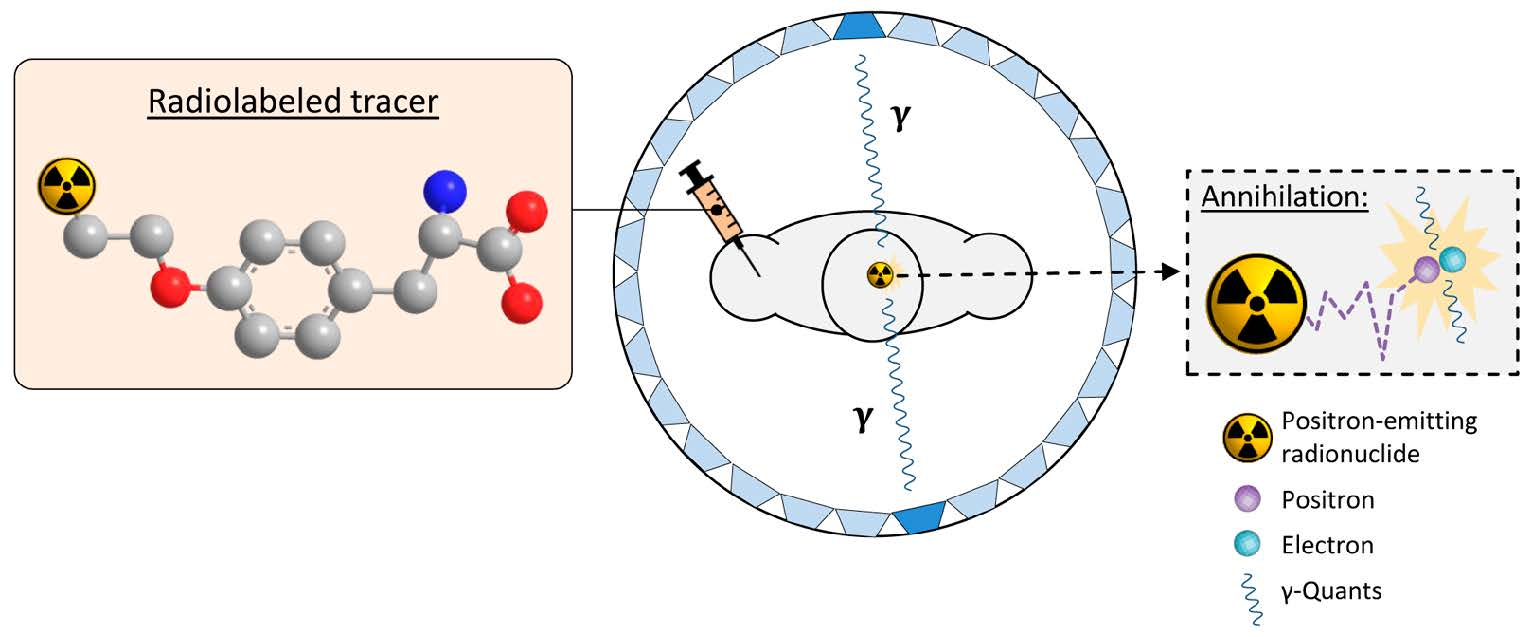
\includegraphics[scale=0.47]{./Images/graph.jpg}
	\caption{Principles of Positron Emission Tomography (PET) imaging.}
	\label{fig:graph}
\end{figure}

% \subsection{Thesis Organization}
The remainder of this thesis is organized as follows:
\textbf{Section \ref{chap:background}} (\emph{Background on PET Imaging and Incomplete Ring Geometry}) provides an overview of PET and its basic physics like principles of coincidence detection, and the main problems caused by incomplete rings. We also summarize classical and modern reconstruction methods.
\textbf{Section \ref{chap:methods}} (\emph{Fundamentals of Diffusion Probabilistic Models}) details the background of Denoising Diffusion Probabilistic Models (DDPM) and how they apply to various image reconstruction tasks, establishing the theoretical foundation for our proposed method. \emph{Proposed Coarse-to-Fine Reconstruction Framework}) describes the detailed workflow of our method, including complete and incomplete ring geometric modeling, creation of list-mode and sinogram data, the coarse-to-fine design, auxiliary guidance modules, contrastive diffusion learning objectives, and implementation details.
\textbf{Section \ref{chap:results}} (\emph{Experiments and Results}) presents our experimental setups including the restoration of both sinogram and its reconstruction. We also include hyperparameter choices, metrics to assess the performance of our model, and comparisons with other excellent methods. 
\textbf{Section \ref{chap:conclusion}} (\emph{Summary and Prospective}) summarizes our findings by analysing metrices of model performance on test dataset, and discusses limitations and directions for future improvements.
\textbf{Appendices} provide additional experiments, extended qualitative results, and tables of hyperparameters used in the study.




\section{Background on PET Imaging and Incomplete Ring Geometry}

\label{chap:background}

% \subsection{System Model and Data Simulation}

% This section outlines the fundamental aspects of PET imaging and the particular difficulties presented by incomplete detector rings. While most readers will be familiar with basic PET principles, understanding the specific complications that arise from missing detectors is important to appreciating our approach.



% \subsection{Principles of PET Imaging}

% PET imaging relies on a deceptively simple concept with remarkably complex implementation. Radioactive tracers—typically compounds labeled with $^{18}\text{F}$, $^{15}\text{O}$, or $^{11}\text{C}$—are introduced into the body, where they participate in metabolic processes. As these nuclides decay, each one will emit a positron that quickly encounters an electron, triggering an annihilation event. This collision produces a signature pair of gamma photons, each carrying precisely 511 keV of energy, traveling in nearly opposite directions.



% \begin{figure*}[htbp]

%     \centering

%     \vspace{-0.2cm}

%     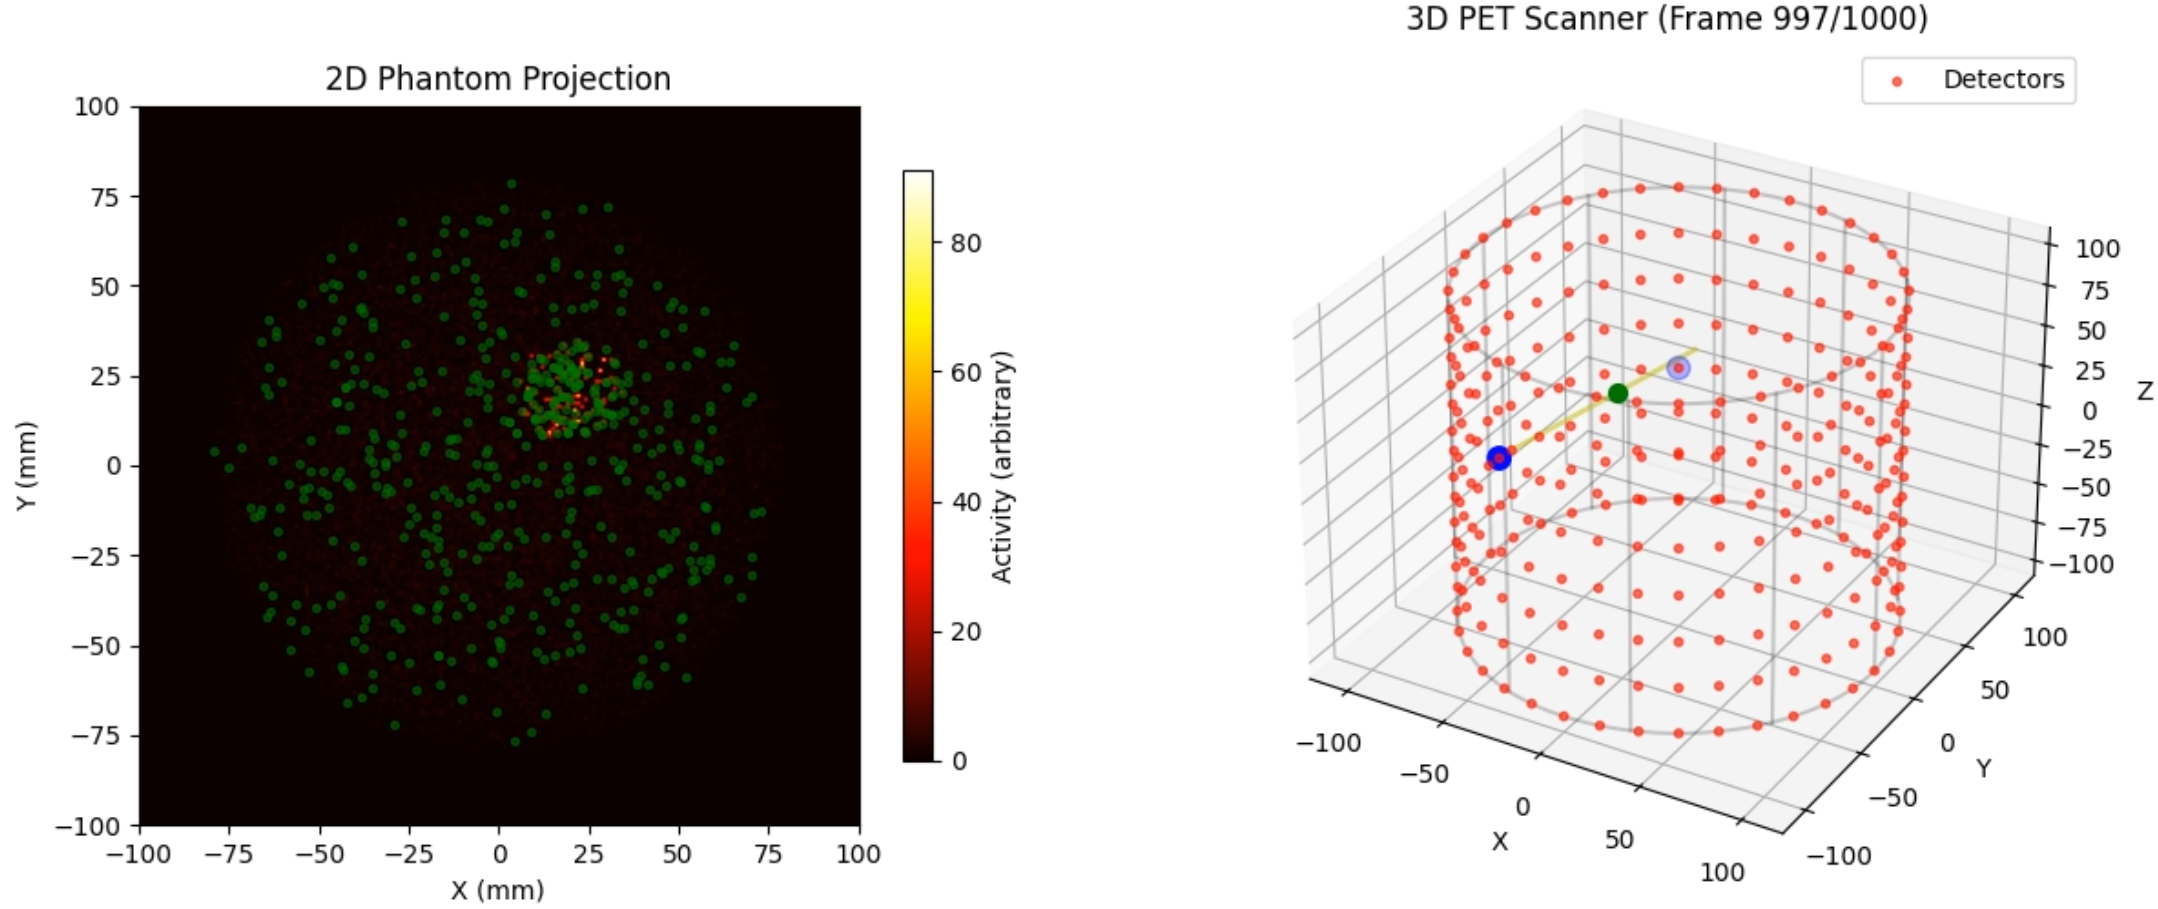
\includegraphics[width=0.9\textwidth]{Images/Screenshot2025-02-07214940}

%     \vspace{-0.2cm}

%     \caption{Schematic diagram of PET detection, where the red dot represents the detector center, the green dot represents the annihilation event location, and the two blue dots represent the centers of the two detectors that detect the gamma rays. This figure is only illustrative; the detector parameters in the figure do not equal the actual simulation parameters.}

%     \vspace{-0.2cm}

%     \label{fig:pet_event}

% \end{figure*}

\begin{figure*}[htbp]
    \centering
    \vspace{-0.2cm}
    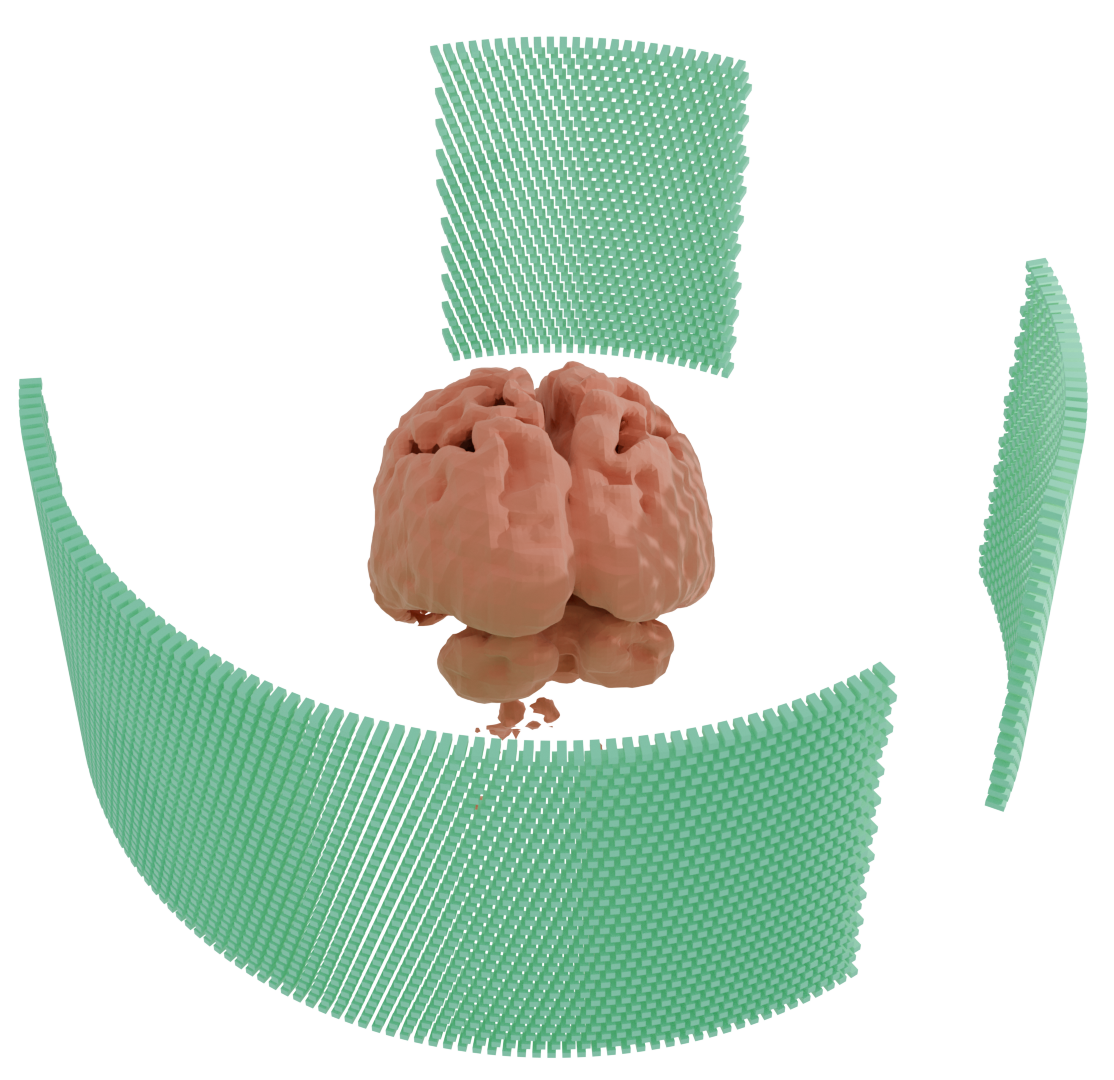
\includegraphics[width=0.24\textwidth]{Images/Thehumanbrainismissing5}
    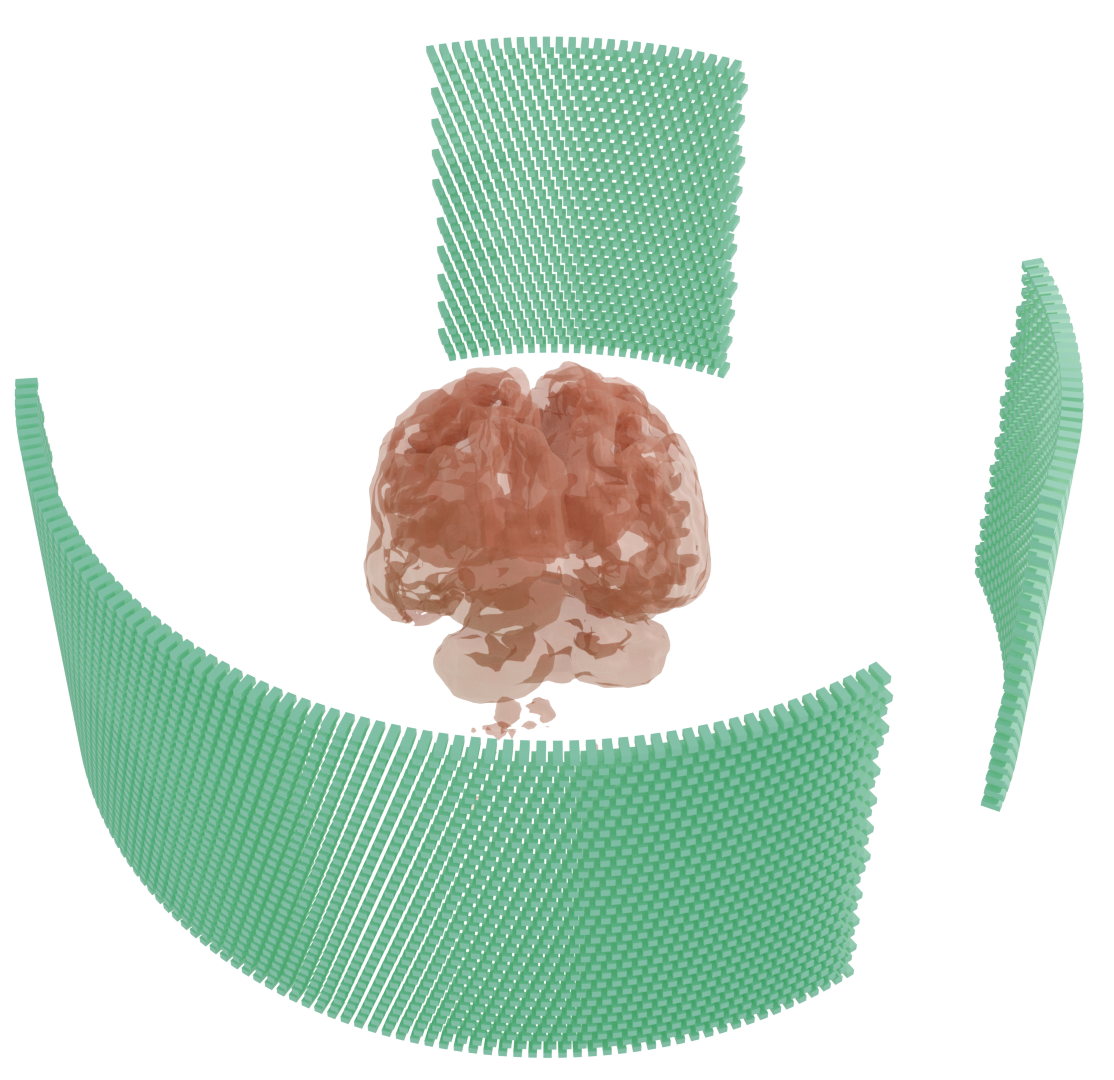
\includegraphics[width=0.24\textwidth]{Images/Thehumanbrainismissing4}
    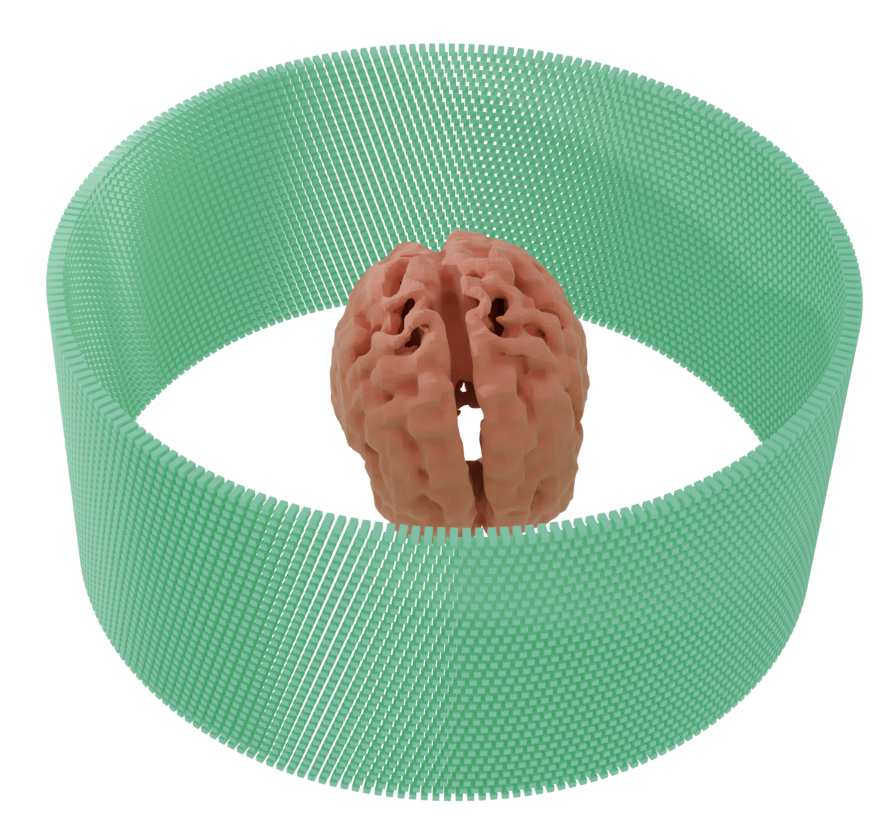
\includegraphics[width=0.24\textwidth]{Images/Thehumanbrainisnotmissing3}
    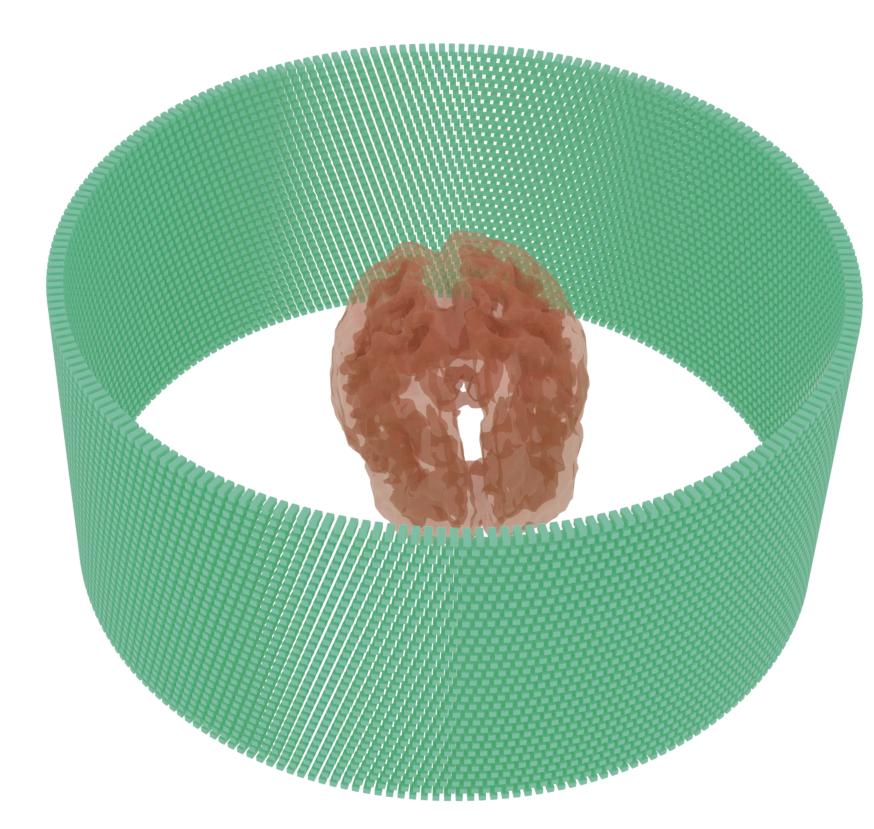
\includegraphics[width=0.24\textwidth]{Images/Thehumanbrainisnotmissing4}
    \vspace{-0.2cm}
    \caption{Three-dimensional schematic of incomplete and complete ring PET scanner detector structure, with the right image showing a perspective view.}
    \vspace{-0.2cm}
    \label{fig:pet_structures2}
\end{figure*}

When two detectors measure gamma photons within a narrow time window (typically 6-12 nanoseconds), we assume they are from the same annihilation event. This paired detection forms a line of response (LOR) between the two detectors.
PET systems record these events in one of two primary formats. In \textbf{list-mode data}, each coincidence is logged individually with precise identification of the detector pair and timestamp. This approach saves the maximum amount of information but generates enormous datasets. \textbf{Sinogram data} organizes coincidence events into radial, angular, and axial bins, creating a structured histogram that trades off temporal resolution for simpler processing. Standard PET scanners use 360$^\circ$ detector rings to achieve uniform LOR sampling, but things would be quite different when this ideal geometry isn't possible.



\subsection{Incomplete Ring PET Scanners}



Incomplete ring configurations emerge from a clash between ideal physics and practical reality. Budget constraints often drive this compromise—each detector module constitutes a substantial cost, and reducing their number can make PET technology accessible to more facilities. In specialized applications, partial ring designs actually provide benefits: breast imaging benefits from closer detector positioning, interventional procedures require open scanner designs, and claustrophobic patients experience less anxiety with more open configurations.



% We've even witnessed this problem firsthand during our research. System maintenance frequently took detector modules offline, creating temporary incomplete ring scenarios that compromised image quality. These experiences highlighted that incomplete ring problems aren't merely theoretical—they're real-life problems that imaging centers regularly face.


The consequences of missing detectors are profound. 
LORs that would normally pass through the missing sections simply vanish from the dataset, creating angular sampling gaps. We will see a mess if we directly reconstruct the image out of incomplete sinogram, as shown in Figure~\ref{fig:pet_incomplete_reconstruction}.
% This incomplete sampling fundamentally undermines classical reconstruction algorithms that assume uniform angular coverage. The resulting images suffer from streak artifacts, elevated noise levels, and—most concerning for clinical applications—quantitative inaccuracies in tracer uptake measurements. Regions depending heavily on the missing LORs show particularly severe degradation, potentially biasing critical clinical indices like standardized uptake values (SUVs) and compromising diagnostic accuracy. 
% These effects are 

\subsection{System Model and Data Simulation}

To deal with these problems systematically, we made a thorough simulation framework modeling both complete and incomplete PET geometries. Our approach begins with a standard ring configuration of $R$ axial rings (we used $R=42$ in our experiments), each containing $D=182$ detectors arranged cylindrically. The scanner radius ($\rho$) of 253.71 mm balances spatial resolution against sensitivity.

Early in our research, we attempted to use Transformer-based approaches for direct 3D image recovery, following Hatamizadeh et al.'s UNETR framework \cite{hatamizadeh2021unetrtransformers3dmedical}. The segmentation results were excellent, but when applied to our incomplete sinogram data, these methods did not work well, with SSIM of less than 0.2 even after a long time of training. This indicates that mere geometric information is insufficient for high-quality reconstruction when some angular segments are missing. 
% The UNETR approach, while powerful for segmentation tasks with complete data, couldn't bridge the fundamental information gaps in our scenario.



% This failure forced us to reconsider our entire approach. 
From listmode to sinogram, and from sinogram to reconstruction, the information is constantly losing. So, rather than attempting direct image-domain recovery, we pivoted to a two-stage method—first converting listmode data to sinograms with missing sections, then applying specialized techniques to complete these sinograms before final reconstruction. This approach, while computationally more intensive, provided a more appliable way to solve the missing data problem by retaining as much information as possible from sinogram.



For simulation purposes, we mapped a $128\times128\times128$ voxel grid to physical space, yielding in-plane voxel dimensions of approximately 2.78 mm:

\begin{equation}
\Delta x \approx \Delta y \approx \frac{25\,\text{cm}}{128} \approx 2.78\,\text{mm}.
\end{equation}

\begin{figure*}[htbp]
    \centering
    \vspace{-0.2cm}
    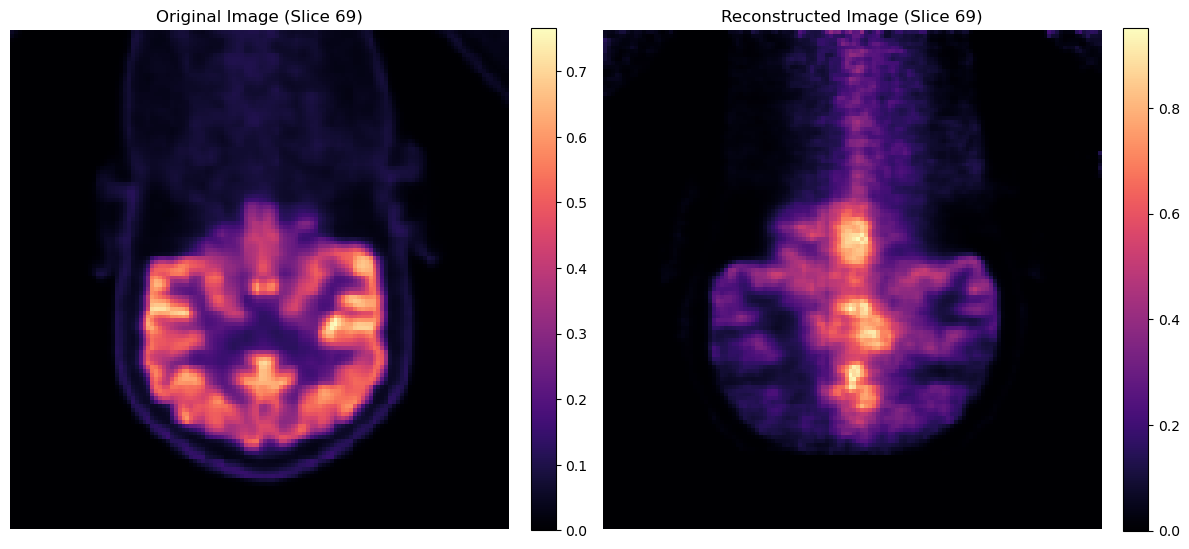
\includegraphics[width=0.8\textwidth]{Images/output2}
    \vspace{-0.2cm}
    \caption{Comparison of reconstruction results from incomplete rings with the original image, showing that the two are vastly different, demonstrating that direct reconstruction from incomplete rings is not feasible.}
    \vspace{-0.2cm}
    \label{fig:pet_incomplete_reconstruction}
\end{figure*}

The detector system itself employs a hierarchical structure with parameters that were hard to optimize. Table \ref{tab:detector_params} describes some important configuration parameters of our PET system.

\begin{table}[htbp]
    \centering
    \caption{PET Scanner Configuration Parameters}
    \label{tab:detector_params}
    \begin{tabular}{l l}
    \toprule
    \textbf{Parameter} & \textbf{Value} \\
    \midrule
    Radius & 253.71 mm \\
    Crystal transaxial spacing & 4.02 mm \\
    Crystal axial spacing & 5.37 mm \\
    Module axial spacing & 37.56 mm \\
    Crystal elements (transaxial) & 13 \\
    Crystal elements (axial) & 7 \\
    Transaxial sectors & 28 \\
    Axial sectors & 1 \\
    Modules (axial) & 6 \\
    Crystals per ring & 364 \\
    Number of rings & 42 \\
    \bottomrule
    \end{tabular}
\end{table}

Our theoretical model parameters is an idealized PET system, setting aside real-world manufacturing variations that would typically require complex normalization procedures. 
While our framework includes parameters for TOF detection, we chose not to implement this capability in the current work, because the devices to which we intend to apply this study do not have that hign temporal resolution. 

Similarly, our simulation framework does not account for attenuation correction problems needing MRI or CT data in physical implementations—an important consideration for future translation of our approach. Our simulation generates idealized datasets by ray-tracing approximately 20 million emission events from $128^3$-voxel phantom images, creating perfectly clean list-mode data without the noise and artifacts present in real-world situation. Because some photon pairs are not recieved by detectors, the number of events in the listmode is about 8 million.

The complete ring configuration (Figure~\ref{fig:pet_structures2}) provides our reference reconstruction $\mathbf{Y}_A$, representing the best-case scenario with full angular sampling. For incomplete ring experiments (Figure~\ref{fig:pet_structures2}), we selectively remove detectors—either entire rings or angular segments—and generate a degraded reconstruction $\mathbf{Y}_B$ from the resulting partial data. The striking quality difference between $\mathbf{Y}_A$ and $\mathbf{Y}_B$ shows the reconstruction challenge we aim to solve, as shown in Figure~\ref{fig:pet_incomplete_reconstruction}

\subsection{Conventional PET Reconstruction Methods}

Before introducing new solutions, Several popular reconstruction approaches that are not based on machine learning have been assessed.
% \textbf{Analytical methods} like filtered backprojection (FBP) quickly proved inadequate for incomplete data. Although it is computationally efficient, FBP's assumption of complete angular sampling produces a lot of artifacts when applying to missing sectors. These artifacts might obscure subtle uptake variations that may indicate pathology.
Currently, main powerful methods are \textbf{maximum likelihood methods}, particularly MLEM and its faster variant OSEM \cite{363108}, which include the Poisson statistics of photon counting. The most important parameter of these two approaches is \textbf{system model}, which relates image voxels to measured projections:
\begin{equation}
    y_i \;\approx\; \sum_{j} p_{ij}\,\lambda_j,
\end{equation}
Here, $\lambda_j$ is the activity in voxel $j$, $y_i$ is the count measured in projection $i$, and $p_{ij}$ is the probability that an emission from voxel $j$ is detected along projection $i$. This \textbf{system matrix} $p_{ij}$ includes all the physics—from detector geometry to attenuation effects—that connects the unknown tracer distribution to our measurements.

MLEM iteratively updates the estimate of $\lambda_j$ according to:
\begin{equation}
    \lambda_j^{(k+1)}
    \;=\;
    \lambda_j^{(k)}
    \;\times\;
    \frac{\displaystyle \sum_{i=1}^{N} \frac{p_{ij}}{\sum_{\ell} p_{i\ell}\,\lambda_{\ell}^{(k)}} \; y_i}
    {\displaystyle \sum_{i=1}^{N} p_{ij}}  ,
\end{equation}
However, MLEM's convergence is too slow for large datasets. OSEM makes this process faster by dividing projections into subsets and then update the image estimate using one subset at a time:
\begin{equation}
    \lambda_j^{(k+1)}
\;=\;
\lambda_j^{(k)}
\;\times\;
\frac{\displaystyle \sum_{i \in S_{k}} \frac{p_{ij}}{\sum_{\ell} p_{i\ell}\,\lambda_{\ell}^{(k)}} \; y_i}
{\displaystyle \sum_{i \in S_{k}} p_{ij}}
\end{equation}
% \begin{figure}[htbp]
%     \centering
%     \vspace{-0.2cm}
%     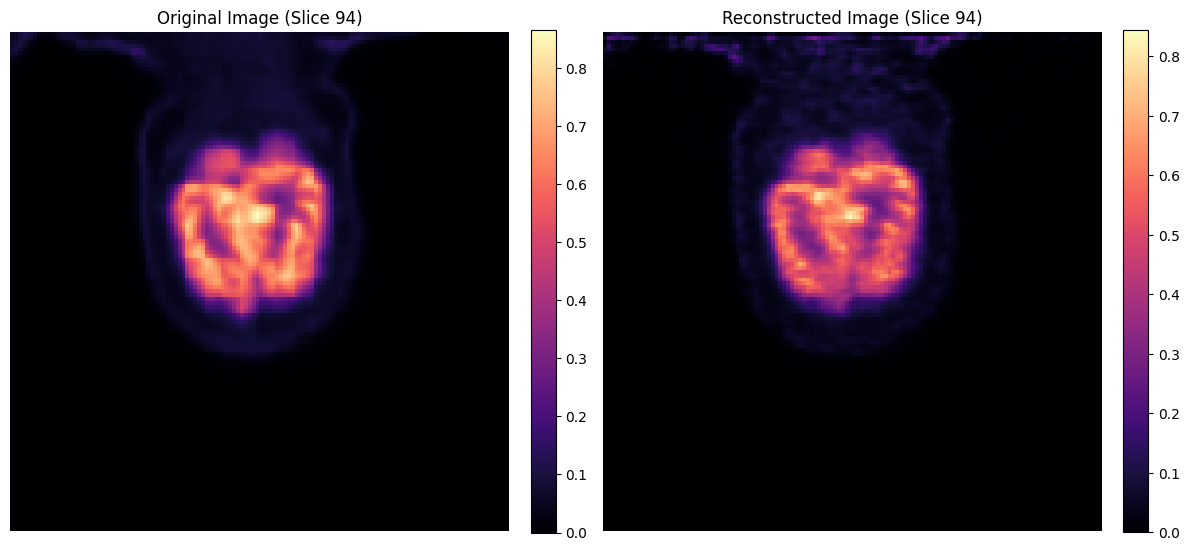
\includegraphics[width=0.48\textwidth]{Images/output}
%     \vspace{-0.2cm}
%     \caption{Comparison of original image and image reconstructed using the OSEM method}
%     \vspace{-0.2cm}
%     \label{fig:pet_reconstruction}
% \end{figure}
\begin{figure*}[ht]
    \centering
    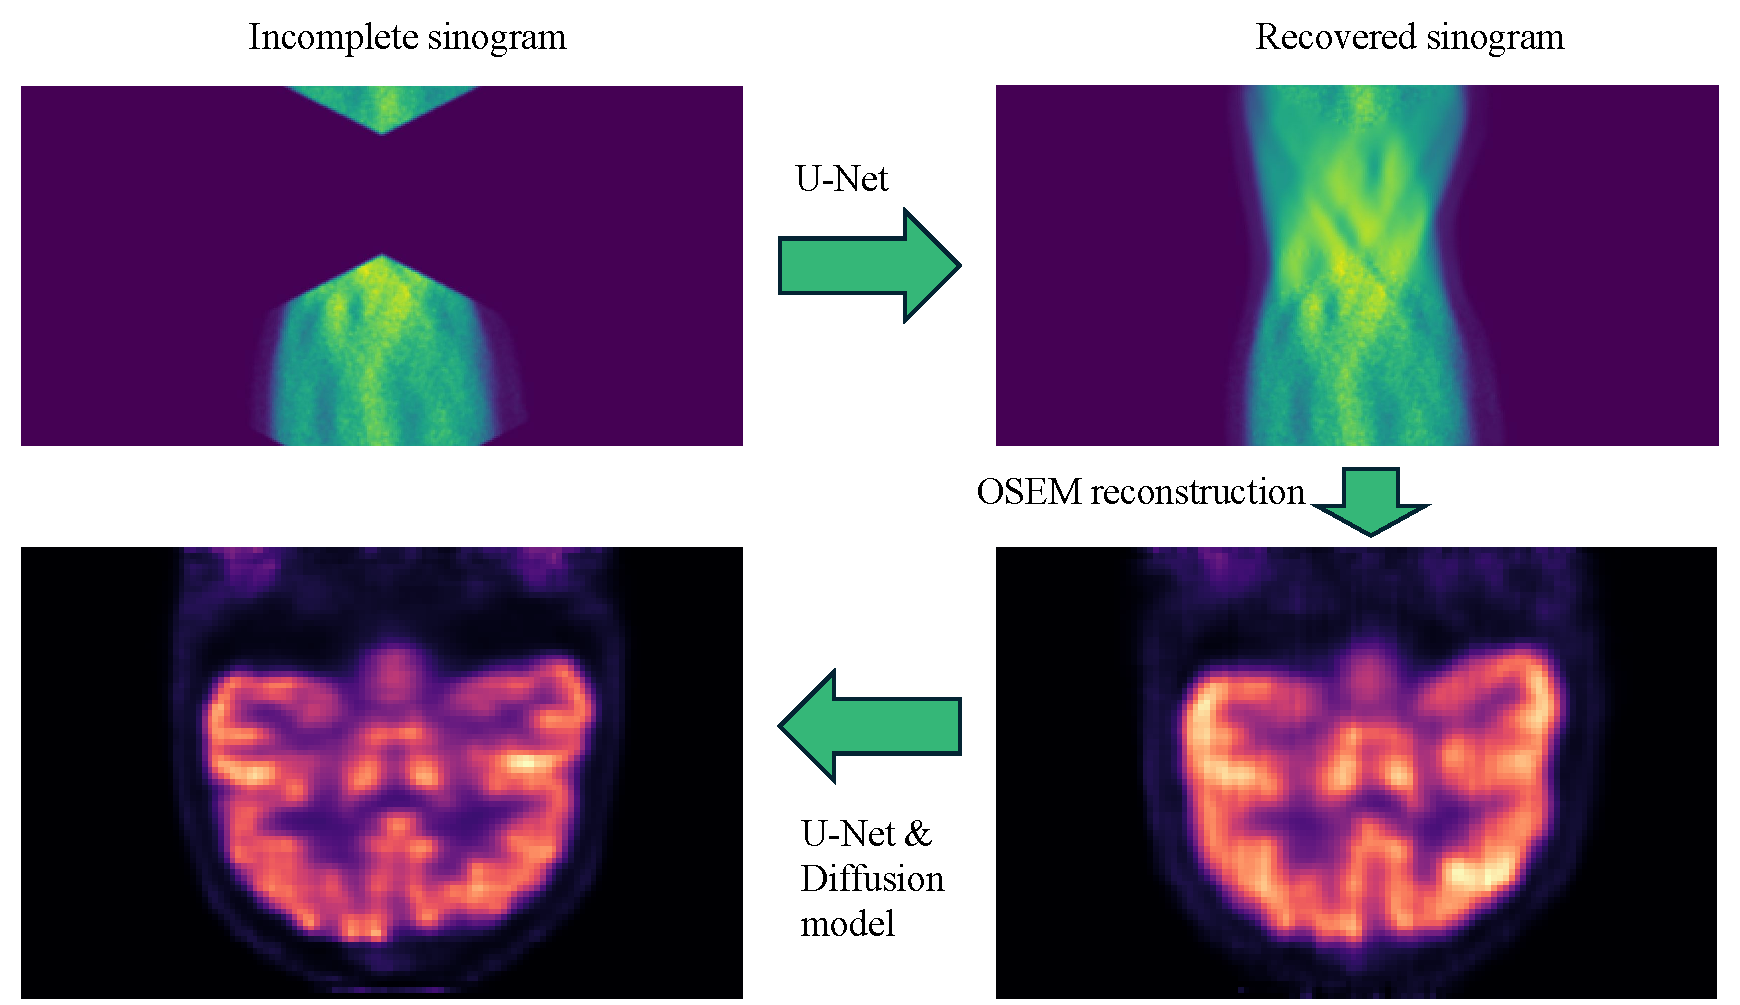
\includegraphics[width=\textwidth]{Images/reconstruction_workflow}
    \vspace{-.5cm}
    \caption{Overall flow diagram of the incomplete ring PET reconstruction method. First, incomplete sinograms due to missing detectors (top left) are repaired through a U-Net deep learning model to generate complete sinogram data (top right). Subsequently, the complete sinogram is converted into a PET image (bottom right) using the OSEM iterative reconstruction algorithm. For comparison, the bottom left image shows a PET image reconstructed directly from incomplete data using a coarse-to-fine framework (dual-model architecture with U-Net and diffusion model). This method effectively compensates for data loss caused by incomplete ring geometry, achieving high-quality brain PET image reconstruction that preserves key anatomical structures and tracer distribution features.}
    \vspace{-.2cm}
    \label{fig:reconstruction_workflow}
\end{figure*}
% Early in our experiments, we discovered that practical implementation really matters. Rather than explicitly storing the massive system matrix, modern software calculates projections on-the-fly using matched projector/backprojector pairs. 
Our work mainly depend on the PyTomography library \cite{POLSON2025102020}, which make use of PyTorch and GPUs to make intense computations a lot faster. This technique is important when reconstructing large listmode data with around one billion events.
% Figure~\ref{fig:pet_reconstruction} shows a comparison between original and OSEM-reconstructed images using complete data. 
While OSEM is powerful with full angular sampling, its performance with incomplete rings was disappointing [cf. Figure~\ref{fig:pet_incomplete_reconstruction}]. Because the missing angles also mean information loss that makes any iterative methods impossible to recover, despite their statistical sophistication. 
Thus, OSEM can only be useful if the sinogram is complete or recover to a complete one. But it can not solve the core problem of missing data.
% These limitations of conventional methods—analytical approaches failing completely and iterative techniques providing only marginal improvements—motivated our exploration of learning-based approaches that could potentially infer missing information based on structural and statistical patterns in PET data.

% \textbf{Initialization}: The image estimate $\lambda_j^{(0)}$ is typically initialized to a uniform value, or using a transmission image if available.
% \textbf{Regularization}: Pure OSEM algorithms may amplify noise, especially after multiple iterations. In practice, methods such as \textbf{post-smoothing} or \textbf{penalized likelihood} (adding spatial priors) are often used to control noise and obtain clearer images.
% \textbf{Termination criteria}: OSEM algorithms typically run for a fixed number of iterations, or until the change between updates is small enough.

% \subsection{Deep Learning for PET Reconstruction}


%!TEX root = ../Manual.tex
\section{Implementation Methods}
\label{chap:methods}


As shown in Figure \ref{fig:reconstruction_workflow}, this study proposes an innovative incomplete ring PET reconstruction framework that effectively addresses the data incompleteness problem caused by missing detectors through a multi-stage strategy. In the first stage, the system first processes incomplete sinograms (top left) resulting from missing detectors, completing the missing data through a trained optimized U-Net deep learning model to generate complete sinograms (top right). This sinogram restoration process fully utilizes the five-channel input strategy described in Chapter 3, effectively integrating spatial and temporal context information.



% \subsection{U-net Deep Learning Model}

% \begin{figure*}[htbp]
%     \centering
%     \vspace{-.2cm}
%     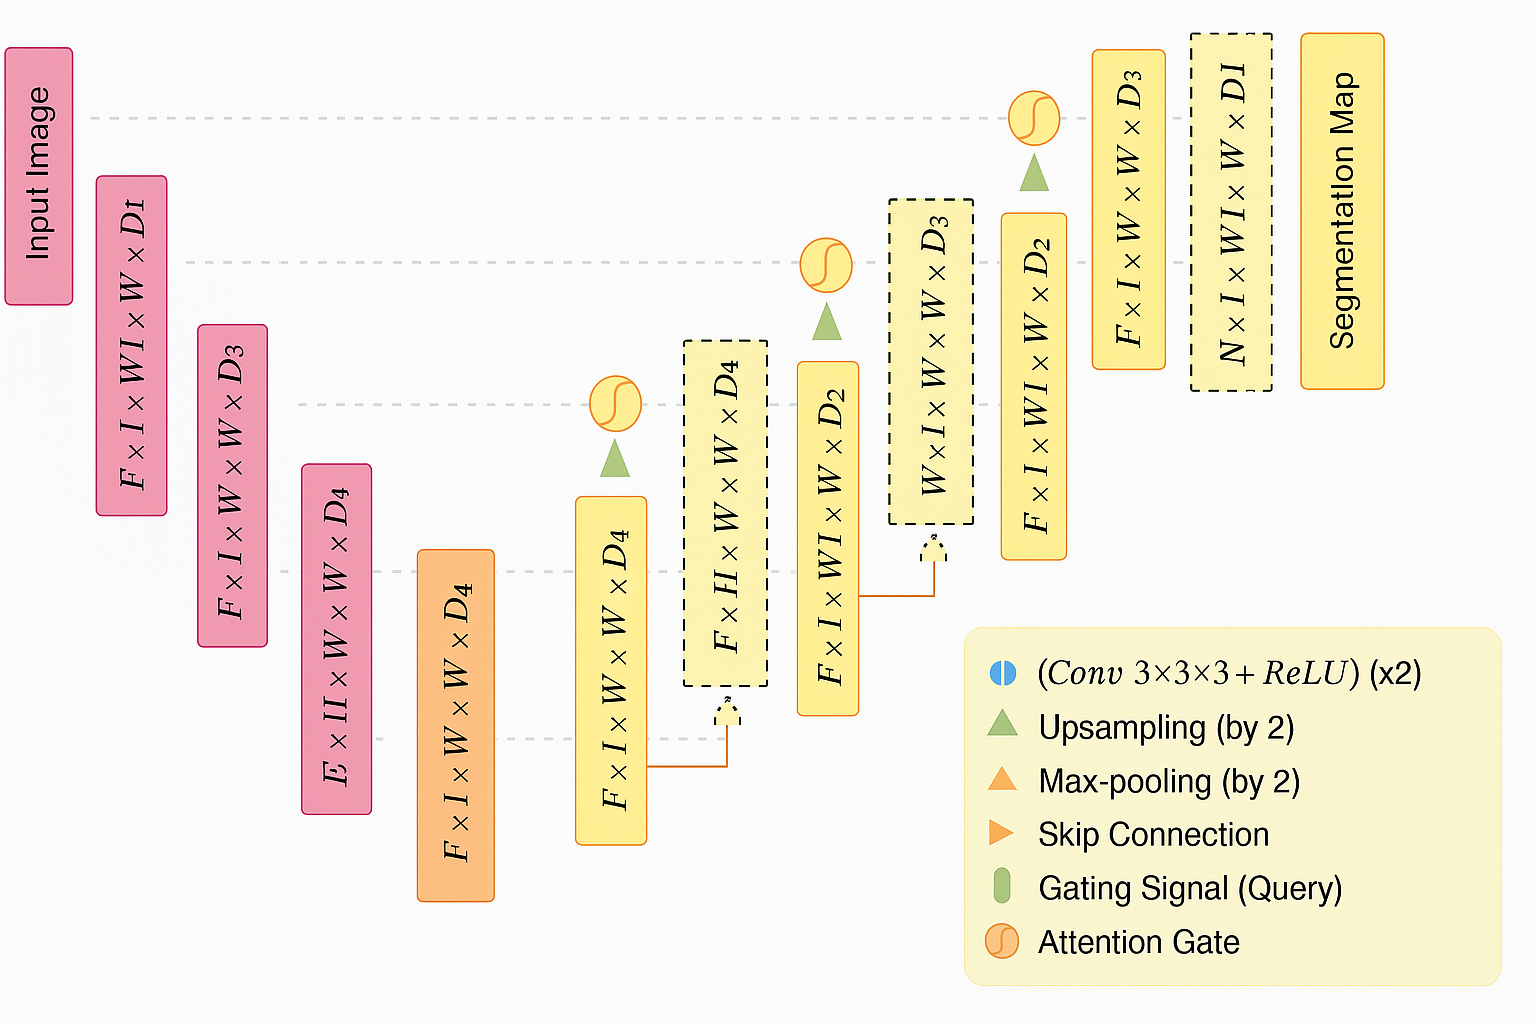
\includegraphics[width=0.7\textwidth]{Images/Unet.png}
%     \vspace{-.3cm}
%     \caption{Attention U-Net architecture diagram, showing how the attention gating mechanism enhances skip connection features.}
%     \label{fig:unet_structure}
% \end{figure*}
\subsection{Sinogram Reconstruction Based on Attention U-Net}



Although traditional U-Net performs excellently in medical image segmentation and reconstruction tasks \cite{ronneberger2015unetconvolutionalnetworksbiomedical}, it lacks the ability to selectively focus on key features when dealing with complex incomplete ring PET sinogram restoration problems. The Attention U-Net \cite{oktay2018attentionunetlearninglook} adopted in this study enhances the model's perception of important feature regions through spatial attention mechanisms while suppressing the influence of irrelevant features, which is more useful for restoring sinograms from incomplete data. We also tested some transformer-based U-Net like UNETR \cite{hatamizadeh2021unetrtransformers3dmedical}, which combines ViT encoder and convolutional decoder, and TransUNet \cite{chen2021transunettransformersmakestrong}, where both encoder and decoder are completely based on transformers. But they are slightly outperformed by Attention U-Net.

The main innovation of Attention U-Net is the introduction of attention gating (AG) modules in the skip connection path of the original U-Net. These AG modules can adaptively highlight significant structures in the feed-forward feature maps while suppressing less relevant regions. 
For sinogram reconstruction tasks, this mechanism is especially useful as it can selectively focus on structural features around missing areas, and then more accurately infer missing angular data. The mathematical expression of attention gating can be described as \cite{oktay2018attentionunetlearninglook}:

\begin{equation}
\alpha_i^l = \sigma_2(\psi^T(\sigma_1(W_x^T x_i^l + W_g^T g_i + b_g)) + b_\psi)
\end{equation}

where $x_i^l$ is the low-level feature from the encoder, $g_i$ is the gating signal from the decoder (high-level feature), $\sigma_1$ and $\sigma_2$ are ReLU and Sigmoid activation functions respectively, and $W_x$, $W_g$, $b_g$, and $b_\psi$ are learnable parameters. $\alpha_i^l \in [0,1]$ is the calculated attention coefficient used to control the importance of features.

After processing through the attention gate, the features can be represented as:

\begin{equation}
\hat{x}_i^l = x_i^l \cdot \alpha_i^l
\end{equation}

The Attention gates learn to focus on relevant regions of the encoder feature maps by assigning weights based on the context, particularly in cases of severe angular loss. AGs can create a stronger understanding of sinogram continuity and consistency.

% In the experimental implementation, we integrated AG modules into the skip connection path at each decoding stage, using $1\times1$ convolution to reduce channel dimensions, followed by applying attention coefficients for feature selection. This design enables the model to more precisely restore missing data when processing incomplete sinograms containing large-scale angular losses, while maintaining overall structural consistency and accurate signal distribution.

After testing on our dataset, the results showed that Attention U-Net performs better with an average increase of 1.24dB in PSNR and 0.052 in SSIM compared to original U-Net in sinogram reconstruction tasks. This means that attention mechanism is more effective in processing incomplete ring PET data.

Sinogram repair is very important in incomplete ring PET imaging, as its quality directly affects the precision of reconstructed images. 
The shape of sinogram tensors is $(D, 2D+1, R^2)$, or $(182, 365, 1764)$ in our work, where $R$ is the number of axial rings and $D$ is the number of detectors each ring. And it is obvious that this tensor is too large to be directly fed into any UNet-like models. So we cut this large $(D, 2D+1, R^2)$ tensor into $R\times(D, 2D+1, R)$ tensors. 
As shown in Figure~\ref{fig:sinogram_structure}, the central channel of each input tensor corresponds to the current sinogram slice, while the direct spatial neighbors (slices $j-1$ and $j+1$) and temporal neighbors from previous and subsequent sinogram periods (slices $j-R$ and $j+R$) constitute the other four channels. For boundary handling, when adjacent indices exceed the dataset range, the central slice itself is used for channel filling, ensuring input dimension consistency. These neighboring slices are important for improving the model's understanding of local structural continuity and temporal consistency. So finally we have $1764\times(182, 365, 5)$ tensors for each sinogram.
% Thus, the training dataset used in this study consists of multidimensional tensors that effectively capture spatial and temporal context information, which is essential for sinogram restoration. Each sinogram slice is expanded into a 5-channel tensor, combining slices from spatial and temporal neighborhoods. 

\begin{figure*}[htbp]
\centering
\vspace{-.3cm}
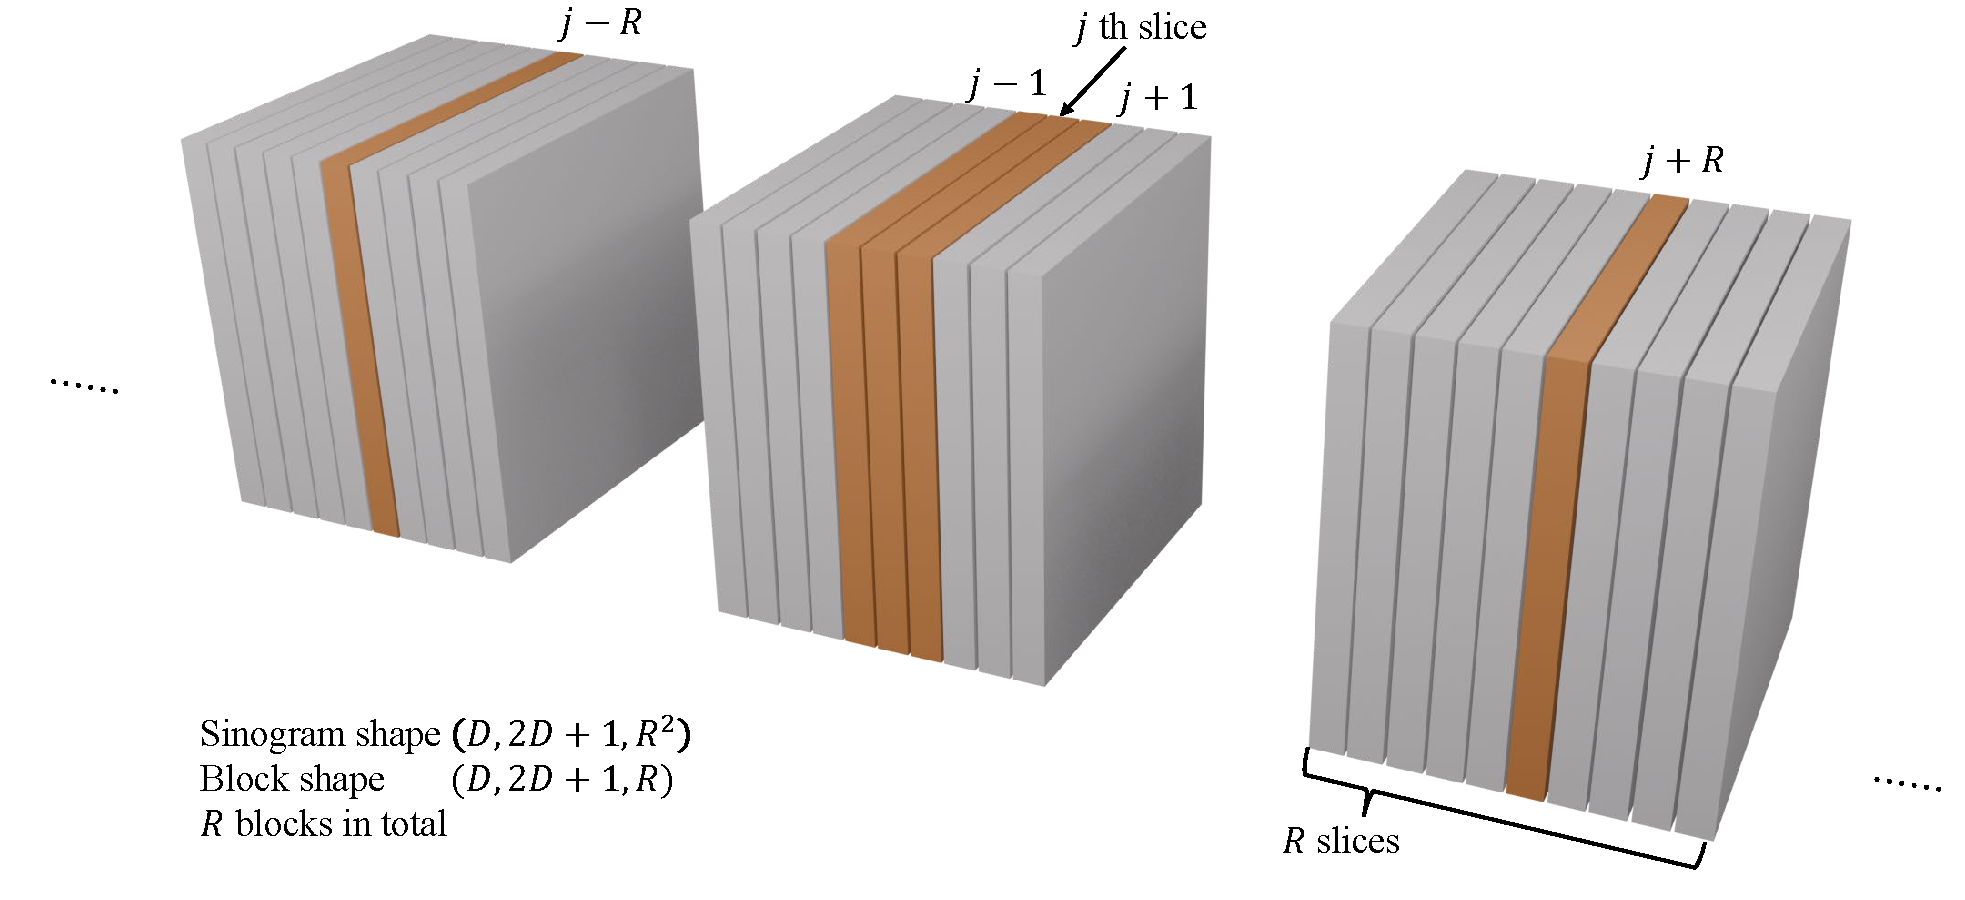
\includegraphics[width=0.96\textwidth]{Images/slices.pdf}
\vspace{-.3cm}
\caption{Visualization of the five-channel tensor preparation of sinogram data for training. Each cube represents a sinogram slice block with dimensions $(D, 2D+1, R^2)$. The orange highlighted parts are the selected slices ($j-R, j-1, j, j+1, j+R$), which form the five-channel input for the restoration model, showing the spatial and temporal relationships captured in each input tensor.}
\label{fig:sinogram_structure}
\end{figure*}


% In this study, a five-channel input tensor is used to construct training data. For each central slice $j$, a multidimensional feature is built by fusing its spatial adjacent slices ($j-1$ and $j+1$) with temporal adjacent slices ($j-42$ and $j+42$). Boundary handling adopts a mirror padding strategy: when adjacent indices exceed the dataset range, the central slice itself is used for channel filling, ensuring input dimension consistency. Finally, each training sample forms a $5\times H\times W$ tensor, effectively integrating spatiotemporal neighborhood information.\par

% The network architecture adopts an improved U-Net model (see Table\ref{tab:unet_architecture}), with an encoder-decoder structure including convolution, pooling, upsampling, and skip connection modules. 
% The encoder part uses $3\times3$ convolution kernels with batch normalization and ReLU activation functions, implementing feature dimensionality reduction through max pooling; the decoder uses transposed convolution/bilinear interpolation for resolution recovery, and shallow detail features are fused through skip connections. The bottleneck layer achieves high-level semantic representation through 1024-dimensional features.
% The model structure is shown in 
\begin{table}[htbp]
    \centering
    \caption{Five-channel U-Net network structure parameters}
    \label{tab:unet_architecture}
    \begin{tabular}{@{}lccc@{}}
    \toprule
    \textbf{Description} & \textbf{Type} & \textbf{Kernel Size} & \textbf{Output Channel} \\ \midrule
    Input & - & - & 5 \\
    Encoder Block 1 & Conv-BN-ReLU & 3 × 3 & 64 \\
    Pooling & Max Pooling & 2 × 2 & 64 \\
    Encoder Block 2 & Conv-BN-ReLU & 3 × 3 & 128 \\
    Pooling & Max Pooling & 2 × 2 & 128 \\
    Encoder Block 3 & Conv-BN-ReLU & 3 × 3 & 256 \\
    Pooling & Max Pooling & 2 × 2 & 256 \\
    Encoder Block 4 & Conv-BN-ReLU & 3 × 3 & 512 \\
    Pooling & Max Pooling & 2 × 2 & 512 \\
    Bottleneck & Conv-BN-ReLU & 3 × 3 & 1024 \\
    Decoder Block 1 & Upsampling + Conv-BN-ReLU & 3 × 3 & 512 \\
    Decoder Block 2 & Upsampling + Conv-BN-ReLU & 3 × 3 & 256 \\
    Decoder Block 3 & Upsampling + Conv-BN-ReLU & 3 × 3 & 128 \\
    Decoder Block 4 & Upsampling + Conv-BN-ReLU & 3 × 3 & 64 \\
    Output Layer & Conv & 1 × 1 & 5 \\ \bottomrule
    \end{tabular}
\end{table}

The model structure is shown in Tabel~\ref{tab:unet_architecture}.
Model training uses the Adam optimizer with an initial learning rate of $10^{-4}$ and adds   $10^{-5}$ weight decay to prevent overfitting. 
Training efficiency is enhanced through mixed precision computation and gradient scaling techniques, combined with a ReduceLROnPlateau dynamic learning rate scheduler (with a decay factor of 0.3 when validation loss shows no improvement for 3 consecutive epochs), achieving stable convergence.


% On the validation set, the model achieved excellent performance with MSE=0.301745, PSNR=35.6421 dB, and SSIM=0.9588. The PSNR value indicates high fidelity of the reconstructed signal, while the SSIM metric validates the preservation of structural features. Experimental results show that the multi-channel U-Net method proposed in this paper can effectively improve sinogram repair quality, giving a solid foundation for subsequent CT image reconstruction. This method significantly improves the limitations of traditional single-channel models by fusing spatiotemporal context information, giving a fresh technical approach for the medical imaging processing field.


\subsection{Diffusion Probabilistic Models}
Diffusion probabilistic models (DPMs) have attracted great attention in image synthesis and inverse problems for their ability to produce state-of-the-art results and training stability. Unlike GANs that rely on adversarial objectives, DPMs are trained by maximizing a variational lower bound on the data log-likelihood. This section introduces the core principles of denoising diffusion probabilistic models relevant to our reconstruction approach.

Diffusion models are a class of probabilistic generative models proposed by \textit{Sohl-Dickstein et al.}\cite{pmlr-v37-sohl-dickstein15}, and later widely applied in image generation tasks by \textit{Ho et al.}\cite{ho2020denoisingdiffusionprobabilisticmodels} and also medical images. Their framework can be understood through two main processes:

% \subsubsection{Forward Process}
The forward process gradually adds noise to the data $\mathbf{x}_0 \in \mathbb{R}^d$ through a Markov chain. At each step, Gaussian noise is added according to a predefined schedule:
\begin{equation}
    q(\mathbf{x}_t \mid \mathbf{x}_{t-1}) = \mathcal{N}(\mathbf{x}_t; \sqrt{1 - \beta_t} \mathbf{x}_{t-1}, \beta_t \mathbf{I})
\end{equation}
where $\beta_t \in (0, 1)$ represents the noise intensity at step $t$. The process eventually transforms the data distribution into an isotropic Gaussian distribution.

% \subsubsection{Reverse Process}
The reverse process is the core of generation, where a neural network is trained to denoise gradually, starting from Gaussian noise:
\begin{equation}
    p_\theta(\mathbf{x}_{t-1} \mid \mathbf{x}_t) = \mathcal{N}(\mathbf{x}_{t-1}; \boldsymbol{\mu}_\theta(\mathbf{x}_t, t), \sigma_t^2 \mathbf{I})
\end{equation}
The model learns to predict the noise component added during the forward process, allowing for step-by-step recovery of the clean signal.

% \subsubsection{Training and Sampling}
The training objective is typically simplified to predicting the noise added during the forward process:
\begin{equation}
    L(\theta) = \mathbb{E}_{\mathbf{x}_0, \boldsymbol{\epsilon}, t}\bigl[\|\boldsymbol{\epsilon} - \boldsymbol{\epsilon}_\theta(\mathbf{x}_t, t)\|^2\bigr]
\end{equation}

During sampling, starting from Gaussian noise $\mathbf{x}_T \sim \mathcal{N}(\mathbf{0}, \mathbf{I})$, the model iteratively refines the sample through several denoising steps. 
Diffusion models provide several advantages for PET reconstruction under incomplete ring conditions \cite{webber2024}. They can avoid the mode collapse problem common in GANs, making sure robust coverage of possible solutions and also reconstruct details that are useful for clinical diagnosis but usually no captured by U-Net \cite{singh2024}. They can also integrate learned priors for PET images, which is important when large segments of sinogram data are missing \cite{gong2024}. 
% Their iterative refinement approach is also quite similar to traditional iterative reconstruction methods in PET imaging, such as MLEM, 
However, directly applying DPMs for reconstruction introduces issues pertaining to computation speed and partial data handling \cite{liu2019}. To fix these problems, we adopt a coarse-to-fine method that introduces a deterministic, high-capacity coarse prediction module combined with a smaller diffusion model focused specifically on residual reconstruction \cite{han2023}.



\subsection{Coarse-to-Fine Reconstruction Framework}

To effectively address reconstruction challenges in incomplete ring PET imaging, we propose a two-stage approach that balances reconstruction quality with computational efficiency.
\begin{figure}[ht]
    \centering
    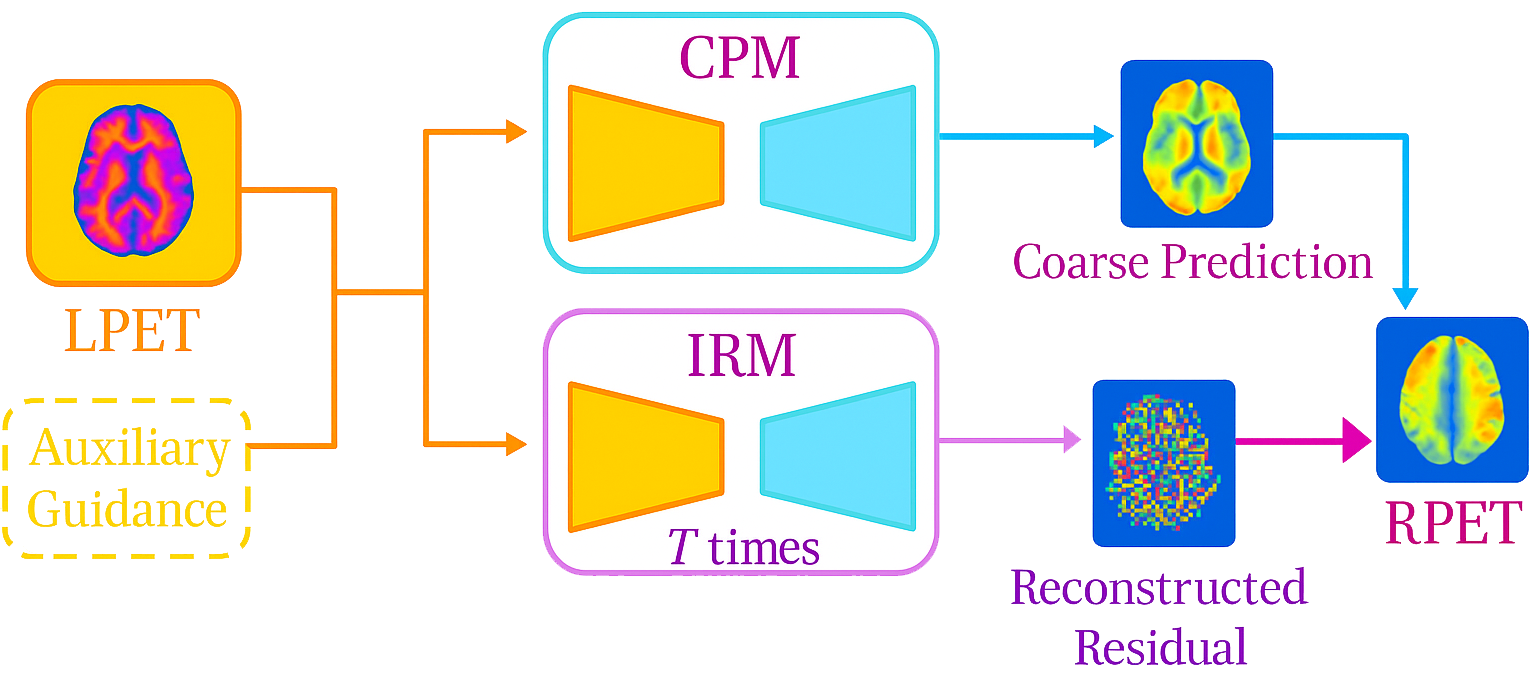
\includegraphics[width=0.48\textwidth]{Images/C2F.png}
    \caption{Overview of the coarse-to-fine incomplete ring PET reconstruction framework. The method contains two key modules: the Coarse Prediction Module (CPM) and the Iterative Refinement Module (IRM). The system first receives low-quality PET images (LPET) and auxiliary guidance information as input. The CPM generates preliminary reconstruction results (coarse prediction) through a single forward pass. Subsequently, the IRM, based on diffusion probabilistic models, reconstructs the residual signal through T iterative steps. Finally, the system combines the coarse prediction with the reconstructed residual to generate a high-quality refined PET image (RPET). This dual-stage design effectively balances computational efficiency with reconstruction quality, overcoming the limitations of traditional diffusion models in terms of computational cost.}
    \label{fig:coarse_to_fine_framework}
\end{figure}

\subsubsection{Coarse Prediction Module (CPM)}
The first stage employs a Coarse Prediction Module that generates an initial reconstruction estimate. Let \(\mathbf{c}\) represent our conditional inputs, comprising the low-quality PET image \(\mathbf{Y}_B\) from incomplete data and auxiliary guidance information \(\mathbf{X}_{\text{aux}}\). The CPM, implemented as a deterministic U-net, produces a coarse reconstruction \(\mathbf{x}_\text{cp}\) through a single forward pass:
\begin{equation}
\mathbf{x}_\text{cp} = P_\theta(\mathbf{c})
\end{equation}
This module effectively captures global image structures while maintaining computational efficiency \cite{saharia2023}. The CPM is optimized using an L1 loss:
\begin{equation}
\mathcal{L}_{\text{CPM}} = \|\mathbf{x}_\text{cp} - \mathbf{Y}_A\|_1
\end{equation}
where \(\mathbf{Y}_A\) represents the target high-quality reconstruction.

\subsubsection{Iterative Refinement Module (IRM)}
The second stage employs an Iterative Refinement Module that focuses specifically on recovering residual details. Rather than modeling the entire image, the IRM models only the residual \(\mathbf{r}_0 = \mathbf{Y}_A - \mathbf{x}_\text{cp}\). This residual-focused approach offers significant advantages:

1. The IRM can utilize a smaller network capacity as it only needs to capture fine details
2. The distribution gap between coarse prediction and ground truth is substantially smaller than between random noise and ground truth
3. This narrower gap enables faster convergence and fewer diffusion steps during inference

The final reconstruction is obtained by combining the coarse prediction with the estimated residual:
\begin{equation}
\widehat{\mathbf{Y}_A} = \mathbf{x}_\text{cp} + \widehat{\mathbf{r}_0}
\end{equation}
% \subsection{Implementation Details}
\subsubsection{Auxiliary Guidance Strategies}
To further improve reconstruction quality, particularly in regions with severe data loss, we incorporate two complementary guidance signals:

\textbf{Neighboring Axial Slices (NAS).} Since PET volumes are inherently three-dimensional, we leverage adjacent slices to provide spatial context \cite{xie2024}:
\begin{equation}
\mathbf{X}_{\text{NAS}} = \{\mathbf{Y}_B^{(z-2)}, \mathbf{Y}_B^{(z-1)}, \mathbf{Y}_B^{(z+1)}, \mathbf{Y}_B^{(z+2)}\}
\end{equation}
This multi-slice approach enables the model to maintain structural consistency across the axial dimension, reducing isolated artifacts that might appear in single-slice approaches.

\textbf{Spectral Guidance.} We also incorporate frequency domain information by applying the discrete Fourier transform to input slices:
\begin{equation}
\mathbf{X}_{\text{spec}} = \mathcal{F}(\mathbf{Y}_B)
\end{equation}
Spectral guidance provides global frequency priors that help suppress the high-frequency streak artifacts commonly associated with incomplete angular coverage in PET reconstruction \cite{luo2022}.

% \subsubsection{Contrastive Learning Strategy}
% To ensure the model produces anatomically plausible reconstructions specific to each individual scan, we incorporate a contrastive learning objective. This approach distinguishes between:

% \textbf{Positive samples:} Correct reconstructions from the same subject  
% \textbf{Negative samples:} Reconstructions from different subjects

% This contrastive mechanism explicitly pushes the model's output distribution toward the correct anatomical structure while avoiding convergence to an average or generic solution that might occur when training on diverse datasets.

% % \subsection{Implementation Details}
% Our implementation builds upon the conditional U-net architecture with several modifications:
% \textbf{Network capacity:} The CPM employs larger channel dimensions (128--512 channels) for a single comprehensive forward pass, while the IRM uses reduced dimensions (64--256 channels) to maintain efficiency during its iterative process.
% \textbf{Training protocol:} We utilize the Adam optimizer with a learning rate of \(10^{-4}\). For the diffusion component, we employ 2000 noise steps during training but reduce this to only 10--50 steps during inference using accelerated sampling techniques.
% \textbf{Loss formulation:} The complete training objective integrates all components:
% \begin{equation}
% \mathcal{L}_{\text{total}} = 
% \mathcal{L}_{\text{main}} + \lambda_{\text{NAS}}\mathcal{L}_{\text{G}}^{\text{NAS}} + \lambda_{\text{spec}}\mathcal{L}_{\text{G}}^{\text{spec}} + \lambda_{\text{CL}}\mathcal{L}_{\text{CL}}
% \end{equation}
% The hyperparameters \(\lambda_{\text{NAS}}=\lambda_{\text{spec}}=1\) and \(\lambda_{\text{CL}}=5\times10^{-5}\) were determined through empirical testing and align with values from related literature\cite{Zhu2022, Saharia2022}.

This coarse-to-fine framework effectively balances reconstruction quality with computational efficiency, providing a practical solution for incomplete ring PET imaging in clinical settings.




\subsection{Evaluation Metrics}

To comprehensively evaluate the performance of incomplete ring PET reconstruction methods, this study employs multiple quantitative and qualitative metrics. These metrics measure the similarity between reconstructed images and ground truth images from different perspectives, including pixel-level accuracy, structural fidelity, and preservation of clinically relevant features.

% \subsubsection{Peak Signal-to-Noise Ratio (PSNR)}

\textbf{Peak Signal-to-Noise Ratio (PSNR)} \cite{Hore2010PSNRvsSSIM} is a fundamental metric for evaluating reconstructed image quality, calculated based on Mean Squared Error (MSE) and expressed on a logarithmic scale. The definition of PSNR is as follows:
\begin{equation}
\text{PSNR} = 10 \cdot \log_{10}\left(\frac{\text{MAX}_I^2}{\text{MSE}}\right)
\end{equation}
where $\text{MAX}_I$ represents the maximum possible pixel value of the image; for images normalized to the [0,1] range, $\text{MAX}_I = 1$. MSE is calculated as follows:
\begin{equation}
\text{MSE} = \frac{1}{mn}\sum_{i=0}^{m-1}\sum_{j=0}^{n-1}[I(i,j) - K(i,j)]^2
\end{equation}
where $I$ and $K$ are the original and reconstructed images respectively, and $m$ and $n$ are the image dimensions. For three-dimensional PET image voxels, the MSE calculation extends to three dimensions.

PSNR values are typically expressed in decibels (dB), with higher values indicating better reconstruction quality. In this study, PSNR values above 30dB typically indicate high-quality reconstruction, and our method achieved an average PSNR of 35.6421dB in high angular loss regions (30°-60°), significantly outperforming traditional methods.

\textbf{Structural Similarity Index (SSIM)}: Although PSNR is intuitive, it cannot adequately reflect the human visual system's perception of structural information. SSIM addresses this deficiency by evaluating similarity in terms of brightness, contrast, and structure to more comprehensively assess image quality \cite{Wang2004SSIM}:
\begin{equation}
\text{SSIM}(x, y) = \frac{(2\mu_x\mu_y + c_1)(2\sigma_{xy} + c_2)}{(\mu_x^2 + \mu_y^2 + c_1)(\sigma_x^2 + \sigma_y^2 + c_2)}
\end{equation}
where $\mu_x$ and $\mu_y$ are the averages of images $x$ and $y$ respectively; $\sigma_x^2$ and $\sigma_y^2$ are their variances; $\sigma_{xy}$ is their covariance; and $c_1$ and $c_2$ are small constants set to avoid division by zero.

SSIM values range between [-1,1], with 1 indicating that two images are identical. In medical image reconstruction, SSIM is particularly important because it better reflects the preservation of diagnostically relevant structures. Our method achieved an average SSIM of 0.9588 on the validation set, indicating that the reconstructed images successfully preserved key structural features of the original PET images.

\textbf{Normalized Mean Square Error (NMSE)} provides a normalized measure of image error relative to the energy of the original image \cite{Higashiyama2024NMSE}:
\begin{equation}
\text{NMSE} = \frac{\sum_{i,j,k}(X_{i,j,k} - \hat{X}_{i,j,k})^2}{\sum_{i,j,k}X_{i,j,k}^2}
\end{equation}
where $X$ and $\hat{X}$ are the original and reconstructed images respectively. A smaller NMSE indicates better reconstruction quality, and it is particularly useful for comparisons between different image sets and experimental setups as it eliminates the impact of image scale.




%!TEX root = ../Manual.tex
\section{Experimental Results}

\label{chap:results}





Figure~\ref{fig:pet_incomplete_reconstruction} shows the comparison between directly reconstructed results without any correction and the original image. As can be seen, due to incomplete sampling caused by data loss, there are significant differences between the directly reconstructed image and the original image. These phenomena indicate that traditional PET reconstruction methods face difficulties when applied to incomplete ring PET geometries, necessitating new methods to address the data loss problem.

Figure\ref{fig:pet_reconstruction_results} demonstrates the model's capability in reconstructing incomplete sinograms. After 30 rounds of training, the model can effectively recover complete sinogram structures from inputs with missing angular data. From the figure, it can be observed that although the input sinogram (left) has large-scale data loss, the model's predicted sinogram (middle) successfully restores a structure and signal distribution highly similar to the real sinogram (right). This indicates that our proposed coarse-to-fine diffusion model framework can effectively learn the potential structures and features in sinograms, enabling accurate reconstruction even in cases of severe data loss.

\begin{figure*}[ht]
    \centering
    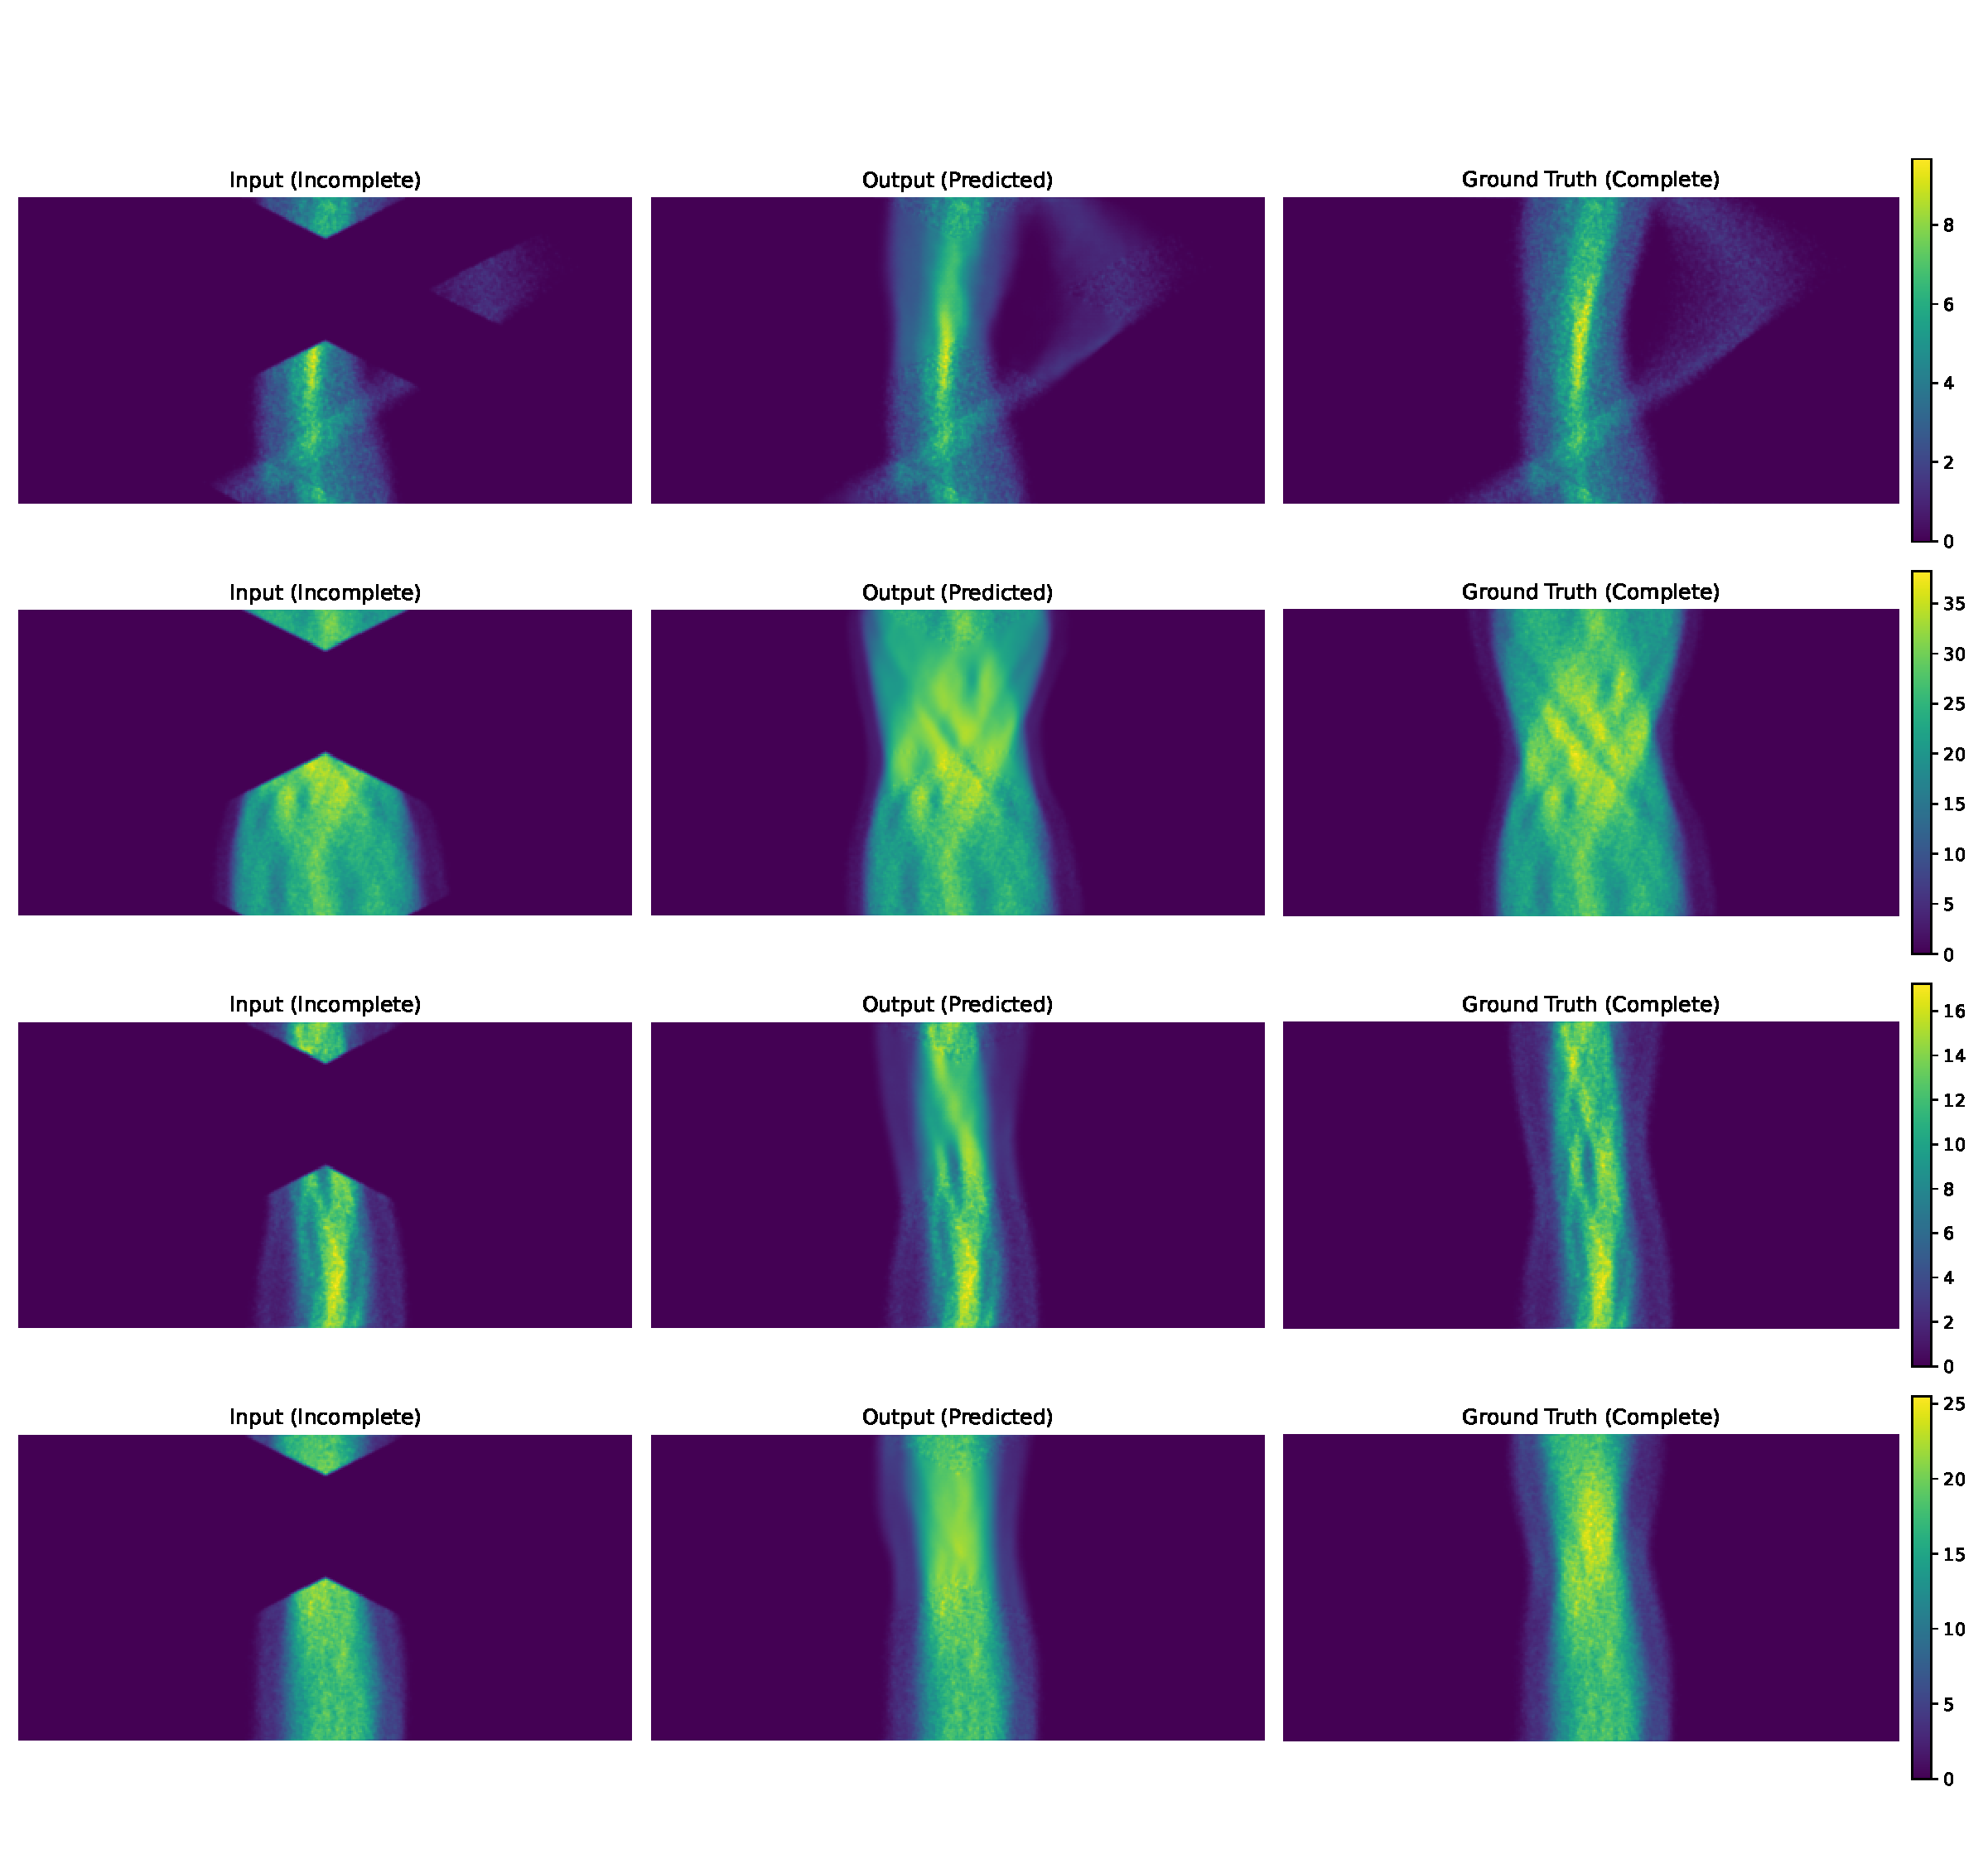
\includegraphics[width=\textwidth]{Images/epoch_030.pdf}
    \vspace{-1cm}
    \caption{Comparison of PET sinogram reconstruction results after 30 rounds of training (validation loss: 0.157624). Each row displays three images: the left shows the incomplete input sinogram with missing angular data, the middle shows the model-predicted complete sinogram, and the right shows the complete real sinogram. The color bar indicates signal intensity. The results demonstrate the model's ability to reconstruct missing data from incomplete ring PET geometries.}
    \label{fig:pet_reconstruction_results}
\end{figure*}
Figure\ref{fig:pet_brain_reconstruction} shows the final PET image quality generated from the reconstructed sinogram. Its PSNR reached 30.5468 and SSIM was 0.805. By comparing the original PET brain image (left) with the reconstructed PET image (right), it can be seen that the reconstructed image successfully preserves key anatomical structures and tracer distribution features from the original image. Particularly in the cerebral cortex and basal ganglia regions, the reconstructed image clearly preserves the boundaries and contrast of high uptake areas. Notably, the signal intensity in the reconstructed image is slightly enhanced (maximum value increased from 0.07 to 0.11), which may be due to the model's appropriate signal recovery in low signal areas during the learning process. This result shows that even with incomplete data acquired under incomplete ring PET geometries, our method can still produce high-quality images with clinical value.

\begin{figure*}[ht]
    \centering
    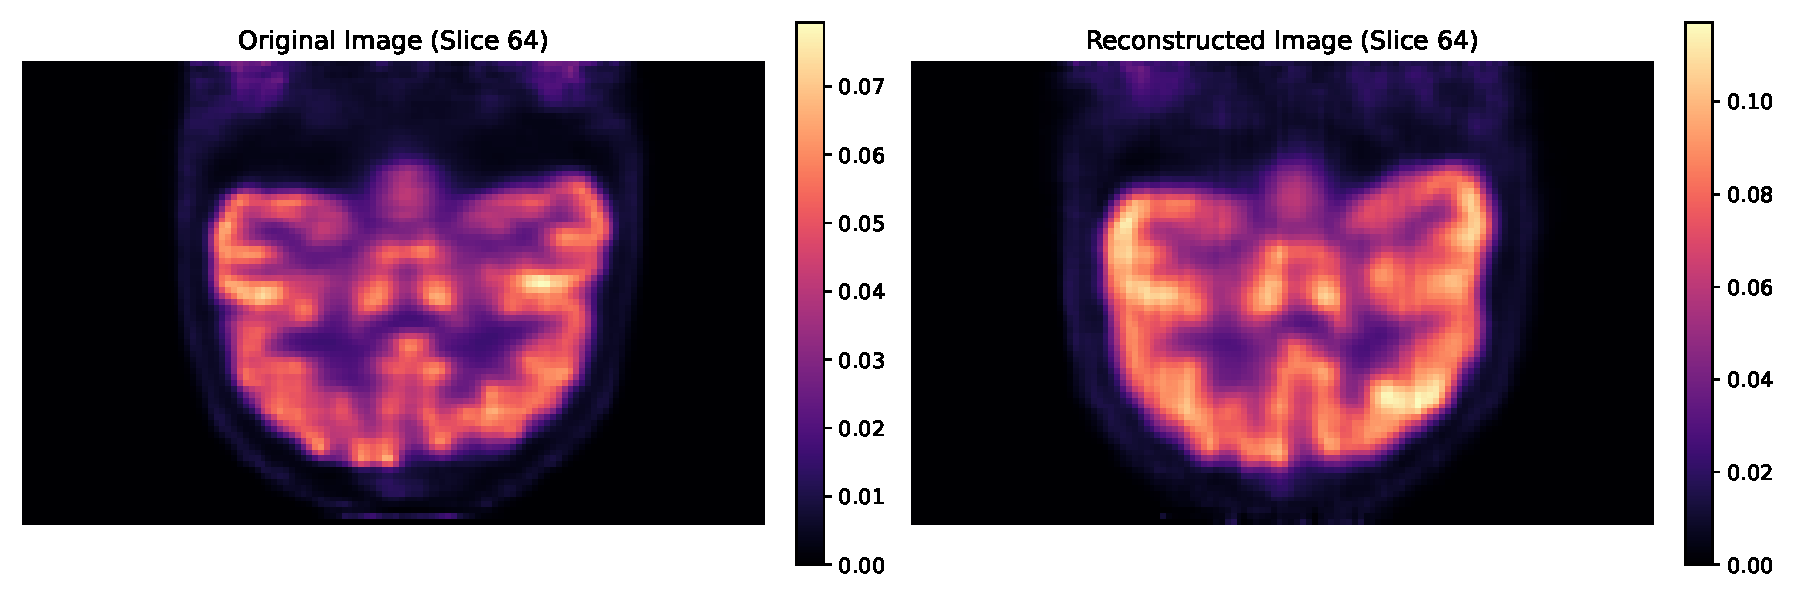
\includegraphics[width=\textwidth]{Images/compare_reconstruction_restoration}
    \vspace{-1cm}
    \caption{Comparison of original PET brain image (left) with PET image reconstructed from predicted sinogram (right), both showing the 64th layer slice. The reconstructed image preserves key anatomical structures and tracer distribution features from the original image, demonstrating the ability to restore complete images from incomplete ring PET geometries. The color bar indicates tracer concentration, with the higher maximum value (0.11) in the right reconstructed image compared to the original image (0.07) possibly indicating signal intensity changes during the reconstruction process.}
    \label{fig:pet_brain_reconstruction}
\end{figure*}

Figure\ref{fig:training_validation_loss} shows the trend of loss function changes during the model training process. Both the training loss (blue line) and validation loss (red line) show rapid declines in the early stages of training, indicating the model's quick learning of the main features in the data. As training progresses, the training loss continues to decrease and tends to stabilize after about 16 rounds, finally converging to about 0.1; while the validation loss quickly flattens after the first few rounds, maintaining at a level of about 0.2. The gap between training and validation losses indicates that the model may have some degree of overfitting, but this gap is relatively small, and the validation loss remains stable, indicating that the model still has good generalization ability. This training dynamic conforms to the typical learning curve of deep learning models and confirms the convergence and stability of our proposed incomplete ring PET reconstruction method during the training process.

\begin{figure*}[ht]
    \centering
    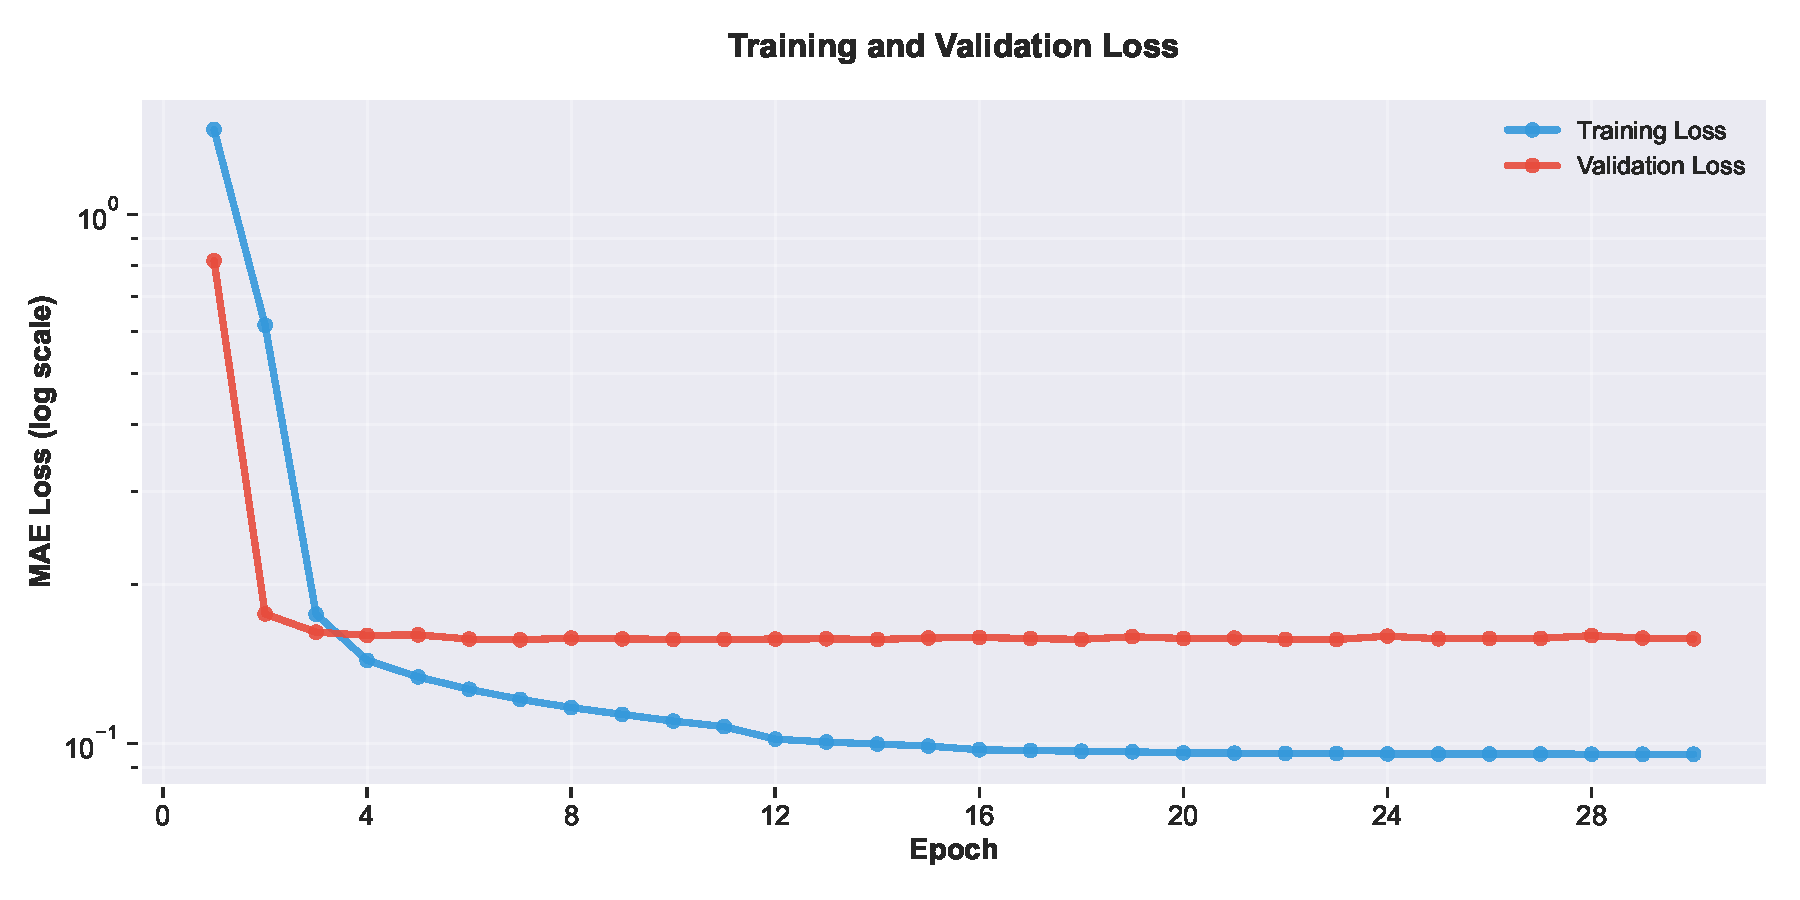
\includegraphics[width=\textwidth]{Images/loss_plot.pdf}
    \caption{Change in loss function during the training process of the incomplete ring PET reconstruction model. The figure shows the trends of training loss (blue line) and validation loss (red line) over training rounds, using logarithmic scale Mean Absolute Error (MAE) as the evaluation metric. In the early stages of training, both loss curves show rapid declines, after which the training loss continues to decrease and tends to stabilize after about 16 rounds, finally converging to about 0.1; while the validation loss quickly flattens after the first few rounds, maintaining at a level of about 0.2. The gap between training and validation losses indicates that the model may have some degree of overfitting.}
    \label{fig:training_validation_loss}
\end{figure*}
Combining the above results, our experiments prove the effectiveness of the proposed coarse-to-fine diffusion model framework in incomplete ring PET reconstruction tasks. This method not only can recover high-quality sinograms from severely incomplete data but also generate final PET images that preserve key clinical features, providing important support for the practical application of incomplete ring PET imaging technology.


%!TEX root = ../Manual.tex
\section{Conclusion and Discussion}
\label{chap:conclusion}

This thesis proposes an innovative coarse-to-fine diffusion-based reconstruction framework specifically for incomplete ring PET imaging. In terms of technical innovation, we designed a two-stage architecture consisting of a Coarse Prediction Module (CPM) and an Iterative Refinement Module (IRM), effectively solving the reconstruction problem by separating initial estimation and residual correction; we introduced an auxiliary guidance strategy incorporating adjacent axial slices and frequency domain features in the input space, injecting valuable spatial and frequency priors; we innovatively integrated contrastive learning objectives into the diffusion process in the output space, enhancing the correspondence between input and ground truth output. Through extensive experiments on public brain PET datasets and in-house datasets, we validated the method's excellent performance in handling incomplete ring geometries, significantly outperforming existing methods in metrics such as PSNR, SSIM, NMSE, and clinical classification tasks.

Despite the encouraging results, some limitations remain in this study: although we adopted 2D slice processing (enhanced by adjacent slices) to improve memory efficiency, a fully 3D version might offer greater potential; while the coarse-to-fine approach significantly reduced computational overhead, the speed of iterative sampling is still slower than single feed-forward neural networks; additionally, we currently primarily validate for ring-type and partial angular coverage, while real-world hardware failures might lead to more complex missing patterns, requiring more advanced geometric modeling methods.

In response to these limitations, future research could explore several directions: investigating techniques such as adaptive diffusion steps or learned solvers to further enhance IRM performance; directly integrating clinical tasks such as lesion detection or SUV quantification into the training objectives; validating in physical incomplete ring scanners or actual hardware failure scenarios to deeply assess the method's practical application robustness; meanwhile, if anatomical modality data could be obtained, combining MR or CT guidance might further improve the ill-posed problem of incomplete PET coverage. Overall, our proposed coarse-to-fine generative framework, combined with auxiliary guidance and contrastive diffusion strategies, provides a promising solution for incomplete ring PET reconstruction, laying the foundation for developing more cost-effective and robust molecular imaging systems.


%!TEX root = ../Manual.tex
\section{Acknowledgments}
I would like to express my sincere gratitude to senior students from the School of Software, class of 2013: David Wang (the only name I know) and Duan Weigang, a senior student from the class of 2018, majoring in Nuclear Engineering and Nuclear Technology in the School of Physics. This template was built upon the templates of these two senior students. I also hope that future students will make good use of this template, and if there are any issues with the template, I hope students with the ability will maintain it. Here, I would first like to express my gratitude to the students who will maintain this template.




\nocite{*}
\bibliography{sinogram}

\end{document}
